\documentclass[12pt]{article}

\usepackage{amssymb}
\usepackage{amsmath}
\usepackage{bm}
\usepackage{color}
\usepackage{float}
\usepackage{graphicx}
\usepackage{mathtools}
\usepackage[none]{hyphenat}
\usepackage{indentfirst}
\usepackage[labelfont=bf]{caption}
\usepackage[left=2.5cm,right=2.5cm, top=2.5cm,bottom=2.5cm]{geometry}
\usepackage{tcolorbox}
\usepackage{lineno}
\usepackage{setspace}
\DeclarePairedDelimiter\ceil{\lceil}{\rceil}

\usepackage[authoryear]{natbib}
\usepackage{hyperref}
\usepackage{yhmath}
\usepackage{accents}

\usepackage{dsfont}
\usepackage{mathtools}
\usepackage{soul}

\overfullrule 5pt

\doublespacing

\usepackage{lipsum}

%\usepackage{adjustbox}
\usepackage{lscape}
\usepackage{afterpage}

\makeatletter
\renewcommand{\maketitle}{\bgroup\setlength{\parindent}{0pt}
\begin{flushleft}
\textbf{\@title}

  \@author
\end{flushleft}\egroup
}
\makeatother

\begin{document}

\linenumbers

\title{A Bayesian Coalescent-informed Model of the DNA Barcode Gap}

\author{Jarrett D. Phillips$^{1, 2*}$ (ORCID: 0000-0001-8390-386X) \\ Nicolas Hubert$^3$ (ORCID: 0000-0001-9248-3377) \\ Robert H. Hanner$^{2}$ (ORCID: 0000-0003-0703-1646) \\
\textit{$^1$School of Computer Science, University of Guelph, Guelph, ON., Canada, N1G2W1} \\ \textit{$^2$Department of Integrative Biology, University of Guelph, Guelph, ON., Canada, N1G2W1} \\ \textit{$^3$UMR ISEM (IRD, UM, CNRS), Universit{\'e} de Montpellier, Montpellier, France}}

\date{}

\maketitle

\vspace{2mm}

\noindent \textbf{*Corresponding Author}: Jarrett D. Phillips$^{1}$

\noindent \textbf{Email Address}: jphill01@uoguelph.ca

\noindent \textbf{Running Title}: Bayesian inference for DNA barcode gap estimation

\noindent \textbf{Word Count}: 9200 (approx.)

\newpage

\begin{abstract}

A simple statistical model of the DNA barcode gap is outlined in both frequentist and Bayesian contexts. Here, accuracy of recently introduced nonparametric metrics, inspired by coalescent theory, is used to characterize the extent of proportional \\ overlap/separation in maximum and minimum pairwise genetic distances within and among species, respectively. Using a straightforward binomial count of overlapping specimen records, probabilities of taxon distance distribution overlap/separation are directly estimated. The mean and variance are derived for edge cases of no and full overlap, and are shown to have good asymptotic properties. Further, a new way to visualize distances and the DNA barcode gap estimators via the empirical cumulative distribution function (ECDF) appears revealing. 

Using R and the probabilistic programming language, Stan, the proposed maximum likelihood estimators (MLEs) and Bayesian model are demonstrated on datasets of 81 \textit{Agabus} diving beetle species sequenced at 3'-COI (36 species), 5'-COI (43 species) and CYTB (two species) mitochondrial gene markers. Analyses clearly expose problems, showing much uncertainty in parameter estimates, particularly under the frequentist paradigm, and when specimen sample sizes for target species are small. Findings herein highlight the promise of the Bayesian approach using a conjugate beta prior for reliable posterior estimation over classical inference when available data are sparse. Obtained results can help shed light on foundational and applied research questions concerning DNA-based specimen identification and species delineation for studies in evolutionary biology and ecology, as well as biodiversity conservation,  forensics, management, and restoration of  wide-ranging taxa.


\end{abstract}

\textbf{Keywords}: Bayesian/frequentist inference, DNA barcoding, Hamiltonian Monte Carlo (HMC), intraspecific genetic distance, interspecific genetic distance, multispecies coalescent, specimen identification, species discovery

\vspace{2mm}

\section{Introduction}

The routine use of DNA sequences to support broad evolutionary hypotheses and \\ questions concerning central demographic processes, like gene flow and speciation, is now ubiquitous. Since the late 1980s, mitochondrial DNA (mtDNA) has been employed to produce a distinctive and measurable signature of genetic polymorphism that readily elucidates \\ phylogeographic patterns, such as colonization, population bottlenecks, and extinction, in diverse and spatially-distributed  taxonomic lineages, like birds, fishes, insects, and \\ arachnids, among other extensively studied groups \citep{avise1987intraspecific}. The application of genomic data to applied fields, like biodiversity forensics, conservation, management, and restoration, for the molecular identification of unknown organismal samples, came later (\textit{e.g.}, Forensically Informative Nucleotide Sequencing (FINS); \citet{bartlett1992fins}). Since its inception over 20 years ago, DNA barcoding \citep{hebert2003biological} built significantly on earlier work and has emerged as a robust method of specimen identification and species discovery across myriad multicellular eukaryotes. This endeavour has dramatically expedited millions of collected specimens to be sequenced at easily obtained short, standardized gene regions like the cytochrome $c$ oxidase subunit I (5'-COI) mitochondrial locus for animals \citep{hebert2003barcoding} in the largest taxon-oriented initiative to date. However, despite now far surpassing the depth and breadth of traditional morphospecies taxonomy at 10 times the speed, and for a fraction of the cost, DNA barcoding is not without its controversies.

The success of the single-locus approach, particularly for regulatory applications, depends crucially on two important factors: (1) the availability of high-quality specimen records found in public reference sequence databases such as the Barcode of Life Data Systems (BOLD; http://www.barcodinglife.org) \citep{ratnasingham2007bold} and GenBank (https://www.ncbi.nlm.nih.gov/genbank/), and (2) the establishment of a DNA barcode gap --- the notion that the maximum genetic distance observed within species is much smaller than the minimum degree of marker variation found among species \citep{meyer2005dna, meier2008use}. Early research has demonstrated that the presence of a DNA barcode gap hinges strongly on extant levels of species haplotype diversity gauged from comprehensive specimen sampling at wide geographic and ecological scales \citep{bergsten2012effect, candek2015dna, chen2022large}. Notwithstanding, many taxonomic groups lack adequate separation in their pairwise intraspecific and interspecific genetic distances due to varying rates of evolution in both genes and taxa \citep{pentinsaari2016molecular}. Furthermore, it has been well-demonstrated that the presence of a DNA barcode gap becomes less certain with increasing spatial scale of sampling, since interspecific distances increase due to population structuring under fragmentation and allopatric divergence, while intraspecific distances \\ shrink as more closely-related species are sampled \citep{phillips2022lack}. This can pose problems in cases of rare singleton species, endemics, or monotypic taxa, for instance \citep{ahrens2016rarity}.  As a result, rapid matching of unknown query samples to expertly-validated references can be compromised, leading to cases of false positives (taxon oversplitting) and false negatives (excessive lumping of taxa) due to incomplete lineage sorting, interspecies \\ hybridization, genome introgression, species synonymy, cryptic diversity, and specimen \\ misidentifications \citep{hubert2015dna, phillips2022lack}. \textcolor{red}{This is because \\ mitochondrial DNA reflects only maternal inheritance; thus, it may not capture the full history of gene flow and divergence across the genome. Discordance between mitochondrial and nuclear signals---due to introgression, incomplete lineage sorting, or sex-biased \\ dispersal---is well documented, and should be considered when interpreting results from DNA barcode gap analyses.} Another culprit includes PCR/sequencing error caused by incorrect nucleotide basecalling, chimeras/heteroplasmies, sample contamination, indels \\ (insertion/deletions), NUMT (nuclear-mitochondrial insert) pseudogene amplification, or \textit{Wolbachia} endosymbiont infection, among other explanations \citep{phillips2023vlf}. Each of these can artificially magnify levels of genetic diversity in taxon populations, rendering techniques like DNA barcoding unreliable for certain groups like marine invertebrates, which are both widely undersampled and possess slow rates of molecular evolution \citep{bucklin2011dna}.

Recent work has argued that DNA barcoding, in its current form, is lacking in statistical rigor \citep{phillips2022lack}. Most publications rely strongly on heuristic distance-based thresholds calculated from convenient specimen sample sizes (usually 5-10 specimens per species, but singletons/doubletons are more prevalent). Instead, focus should be placed on employing optimal sampling designs using collated taxon haplotype information, coupled with knowledge of project funding and budget constraints \citep{phillips2015exploration, phillips2019incomplete, phillips2020hacsim}. This is necessary to accurately infer taxonomic identity and delineate boundaries on the basis of clustering genetic variation into putative groups reminiscent of species \citep{ phillips2022lack}. Of these studies, few report measures of uncertainty, such as standard errors (SEs) and confidence intervals (CIs), around estimates of intraspecific and interspecific variation (\textit{e.g.}, \citet{wiemers2007does}), calling into question the existence of a true species' DNA barcode gap \citep{candek2015dna, phillips2022lack}. To support this idea, novel nonparametric locus- and species-specific metrics \textcolor{red}{informed by} the multispecies coalescent (MSC) were recently outlined by \citet{phillips2024measure} (see \textbf{Methods}). 

The basic coalescent \citep{kingman1982coalescent, kingman1982genealogy} encompasses a backwards continuous-time \\ stochastic Markov process of allelic sampling among lineages under the infinite sites model of mutation within a large neutrally-evolving, panmictic, diploid species population of constant size (\textit{i.e.}, obeying Wright-Fisher dynamics) from the present into the past towards the most recent common ancestor (MRCA). Although the coalescent sampling process plays a foundational role in evolutionary biology and population genetics theory, due to its inherent simplicity and flexibility \citep{rosenberg2002genealogical, degnan2009gene}, the approach has been both under-utilized and under-appreciated as a key player within DNA barcoding \citep{collins2014known, dowton2014preliminary, hubert2015dna, phillips2022lack}. Because mitochondrial markers are haploid, they possess considerably smaller effective population sizes ($N_e$) compared to diploid loci. As a result, regions like COI accumulate diagnostic species-specific mutations at a much faster rate due to fixation by genetic drift \citep{hubert2015dna, phillips2022lack}.  Previously proposed MSC algorithmic approaches (of which there are too many to exhaustively list here, and which have mostly been applied to multilocus sequence data), generally assume either a strict or relaxed molecular clock and a simplified model of DNA nucleotide substitution across closely-related taxa \citep{ho2014molecular, flouri2022bayesian}. From here, an estimated species phylogeny may be easily constructed \textcolor{red}{(\textit{e.g.}, with or without use of a guide tree; \citet{rannala2003bayes, rannala2017efficient, yang2010bayesian, yang2014unguided, yang2017bayesian})}. Even tree- and network-based taxon delimitation methods designed for single loci, such as the Generalized Mixed Yule Coalescent (GMYC) \citep{pons2006sequence, monaghan2009accelerated, fujisawa2013delimiting}, Poisson Tree Processes (PTP) \citep{zhang2013general, kapli2017multirate}, and statistical parsimony/haplotype networks (\textit{e.g.}, TCS networks \citep{templeton1992cladistic}, haplowebs \citep{dellicour2015delimiting, dellicour2018hitchhiker}), which see much use in DNA barcoding initiatives, have their flaws since they depend on strong parametric assumptions which generally do not hold in practice (\textit{e.g.}, Yule birth process). Optimal performance of these methods relies heavily on careful parameter selection (\textit{e.g.}, prior  specification of branching rates in ultrametric trees in the case of GMYC, or the probability of parsimony for nested clade analysis (NCA; \citet{templeton1998nested}), to name a few) \citep{hubert2024delimiting} within third-party software like \textcolor{red}{BEAST2} \citep{bouckaert2019beast}, among other concerns \citep{talavera2013factors, tang2014effects, fonseca2021gmyc}. 

\citet{hubert2024delimiting} categorized statistical species delimitation methods according to five crucial factors necessary for success: availability, reliability, scalability, understandability, and usability. It is proposed herein that this scheme applies equally to the task of specimen identification.  Any proposed identification or delimitation approach should score high across all of these aspects \citep{hubert2024delimiting}. Yet, numerous tradeoffs exist, and so current methods fall short. (See Table 1 in \citet{hubert2024delimiting} for a comprehensive overview.) Careless parameterization of established approaches by users unfamiliar with their underlying statistical characteristics may severely bias overall results in unintended ways \citep{hart2007things}, even if default settings are employed. In contrast, the estimation of DNA barcode gaps has largely been left unexplored from an analytical perspective and currently awaits the development of MSC-based models to handle uncertainty in DNA barcode gap estimation. The approach proposed by \citet{phillips2024measure} and extended herein is both tree- and network-free, and does not require judicious parameter setting; all that is needed is either an upper- or lower-triangular distance matrix. It is similar in requirements to algorithms such as Automatic Barcode Gap Discovery (ABGD) \citep{puillandre2011abgd} and Assemble Species by Automatic Partitioning  (ASAP) \citep{puillandre2021asap}, which have both been rigorously tested under various coalescence scenarios. Therefore, the method is easy to use and interpret, quite memory efficient, very fast to run on large datasets, and archived freely online through GitHub (\href{https://github.com/jphill01/DNA-Barcode-Gap-Coalescent}{https://github.com/jphill01/DNA-Barcode-Gap-Coalescent}). Most importantly, the method ranks highly across all criteria mentioned by \citet{hubert2024delimiting}. 

The estimators from \citet{phillips2024measure} represent a clear improvement over simple, yet arbitrary, distance heuristics such as the 2\% rule noted by \citet{hebert2003biological} and the 10$\times$ rule \citep{hebert2004identification}. The 2\% rule asserts that DNA barcodes differing by at least 2\% at sequenced genomic regions should be expected to originate from different biological species. In contrast, the 10$\times$ rule suggests that barcode sequences displaying 10 times more genetic variation among species than within taxa is suggestive of a distinct evolutionary origin. However, even though DNA barcoding has moved away from relying solely on the use of arbitrary genetic distance thresholds to facilitate specimen identification and species delimitation tasks, through the use of proxies like Molecular Operational Taxonomic Units (MOTUs) via the Barcode Index Number (BIN) framework \citep{ratnasingham2013bin} for instance, the lack of adoption of an explicit and universally agreed-upon species concept in DNA barcoding studies is still missing. The ideal concept is one that readily governs lineage formation and proliferation necessary to establish rigorous taxon definitions for successful delimitation of hypothesized and heuristic evolutionary units using DNA barcode \\ identification criteria \citep{dequeiroz2007species, pante2016species, rannala2015art, wells2022species}. Such a concept must be proposed in conjunction with secondary lines of evidence (\textit{e.g.}, morphology, ecology, geography, ontegeny, phenology, life history, and behaviour) promised by an integrative framework \citep{dayrat2005towards}. This is the case, for instance, with species existing in allopatry/sympatry, where establishment of reproductive isolation on the basis of fixed diagnostic differences using the Biological Species Concept (BSC) \citep{mayr1942systematics}, is challenging \citep{fujita2012coalescent}. Notably, \citet{fujita2012coalescent} remarks that the MSC applied to the taxon delimitation problem harmonizes many species concepts since it identifies independent evolutionary trajectories under the umbrella of the General Lineage Concept. This makes the MSC a fitting tool to model speciation and other modes of diversification \citep{collins2014known}. In addition, the reliance on visualization approaches, such as frequency  histograms, dotplots, and quadrant plots, to expose DNA barcoding's limitations, has also been criticized since they can fog real species signal relative to noise \citep{collins2013seven, phillips2022lack}. Up until the work of \cite{phillips2024measure}, the majority of studies (\textit{e.g.}, \citet{young2021macer}) have treated the DNA barcode gap as a binary response. Given poor sampling depth for most taxa, a Yes/No dichotomy is inherently flawed because it can falsely imply a DNA barcode gap is present for a taxon of interest when in fact no such separation in genetic distances exists. On the other hand, in the case of sequence overlap, while the presence \textcolor{red}{of} a single specimen record is a necessary requirement to nullify the existence of a DNA barcode gap in light of available genetic data, it is not a sufficient condition, since said taxon record could represent a species misidentification or other error. Thus, the MSC serves as an ideal model to settle ongoing debates and issues regarding DNA barcoding's use as both a molecular identification and delineation tool. The recently introduced DNA barcode gap metrics go some way into further operationalizing this task.

A key innovation of the new DNA barcode gap metrics is that they position  DNA barcode gap estimation in a continuous (\textit{i.e.}, probabilistic) light, as opposed to a discrete, deterministic one. More clearly, the DNA barcode gap statistics permit an estimate of distance overlap/separation to be calculated for each considered species within a genus separately and independently at a local scale, rather than at a global scale for the  genus (or higher level taxonomic grouping, such as order or family) as a whole. Exclusive focus on global DNA barcode gaps can be seen in many studies devoted to DNA barcode gap detection (\textit{e.g.}, Lycaenidae: \citet{wiemers2007does}, Annelida: \citet{kvist2014does}, Odonata: \citet{koroiva2018estimating}). Further, the proposed estimators extended herein reinforce the importance of distinguishing between global and local DNA barcoding gaps, which was previously argued by both \citet{collins2013seven} and \citet{phillips2022lack}. \citeauthor{phillips2024measure}'s (\citeyear{phillips2024measure}) proposed statistics quantify the extent of asymmetric directionality of proportional distance distribution overlap/separation for species within well-sampled taxonomic genera based on a \\ straightforward distance count, in a similar vein to established measures of statistical \\ similarity such as the Kullback-Leibler (KL) divergence \citep{kullback1951information} and other related statistics. The metrics can be employed in a variety of ways, including to validate performance of marker genes for specimen identification to the species level (using nonparametric bootstrapping \citep{efron1979bootstrap}, as in \citet{phillips2024measure}). The estimators can further be utilized to assess whether computed values are consistent with fundamental population genetic-level parameters like $N_e$, mutation rate ($\mu$), migration rate ($m$), and divergence time ($\tau$), as well as derived ones, such as the population mutation rate, \\ $\theta = 4N_e\mu$, and the fixation index, $F_{ST}$. This is especially true for species under study within a statistical phylogeographic setting \citep{knowles2002statistical, knowles2004burgeoning, knowles2009phylogeo, mather2019practical}. Early on, species discovery using DNA barcoding was presumed to only work for reciprocally monophyletic groups, and thus concerned itself with terminal branches of generated phylogenies rather than more basal lineages occurring deeper in hypothesized species trees \citep{fujita2012coalescent, mutanen2016species}. Furthermore, the occurrence of short branches and large $N_e$ within resolved phylogenies increases the likelihood of deep coalescence \citep{degnan2009gene}, clouding species  delimitations, which often fail or are uncertain in broad parameter space \citep{hickerson2006dna, carstens2013how, rannala2015art}. As DNA barcoding is a single-locus approach, it is problematic for evolutionarily young taxa. Incomplete lineage sorting within gene genealogies, leading to the retention of ancestral polymorphisms within populations, is a common phenomenon due to the ongoing stochastic dynamic of mutation generating population variation, and genetic drift driving gene variants to fixation \citep{degnan2009gene, rannala2015art}. The most promising way forward in assessing the validity of \citeauthor{phillips2024measure}'s (\citeyear{phillips2024measure}) method seems to be through the use of software such as BPP (Bayesian Phylogenetics and Phylogeography), which permits efficient full Bayesian simulations under various MSC models (\textit{e.g.}, MSC-I (MSC with introgression; \citet{flouri2020bayesian}) or MSC-M (MSC with migration; \citet{flouri2023efficient}), among others) using Markov \textcolor{red}{chain} Monte Carlo (MCMC) for tree parameter estimation (via the {\tt A00} option, for instance) \citep{flouri2018species}, or PHRAPL (Phylogeographic Inference using Approximate Likelihoods) \citep{jackson2017species, jackson2017phrapl}, which employs tractable phylogenetic likelihood \\ calculations via the \textcolor{red}{Genealogical Divergence Index (gdi)}. Other hypothesis-driven approaches to species delimitation model selection, like Bayes Factors (BFs) \citep{leache2014species} and Approximate Bayesian Computation (ABC) \citep{camargo2012species}, are also possible. \\ Rigorous statistical methodology has been historically integrated into DNA barcoding \\ previously \citep{matz2005likelihood, nielsen2006statistical}, though strictly for the purpose of specimen identification. \citeauthor{phillips2024measure}'s (\citeyear{phillips2024measure}) approach is unique as it also greatly extends usage to delimit species, while still being grounded strongly in evolutionary theory: if pairs of species show consistently high values (close to one) of the DNA barcode gap metrics (See \textbf{Methods} for mathematical formulae), this could be suggestive of insufficient taxon boundaries. In such cases, specific species hypotheses could be proposed and explicitly tested, given other supporting evidentiary data. 

While introduction of the new metrics is a step in the right direction, what appears to be missing is a rigorous statistical treatment of the DNA barcode gap. This includes an unbiased way to compute the statistical accuracy of \citeauthor{phillips2024measure}'s (\citeyear{phillips2024measure}) estimators arising through problems inherent in frequentist maximum likelihood estimation for probability distributions having bounded positive support on the closed unit interval [0, 1]. To this end, here, a Bayesian model of the DNA barcode gap coalescent is introduced to rectify such issues. The model allows accurate estimation of posterior means, posterior standard deviations (SDs), posterior quantiles (\textit{e.g.}, median) and \textcolor{red}{Bayesian credible intervals (BCIs)} for the statistics given datasets of intraspecific and interspecific distances for species of interest.

\section{Methods}

\subsection{DNA Barcode Gap Metrics}

The novel nonparametric maximum likelihood estimators (MLEs) of proportional \\ overlap/separation between intraspecific and interspecific distance distributions for a given species ($x$) to aid assessment of the DNA barcode gap are as follows:

\begin{align}
p_x &= \frac{\#\{d_{ij} \geq a\}}{\#\{d_{ij}\}} \\[1mm]
q_x &= \frac{\#\{d_{XY} \leq b\}}{\#\{d_{XY}\}} \\[1mm]
p'_x &= \frac{\#\{d_{ij} \geq a'\}}{\#\{d_{ij}\}} \\[1mm]
q'_x &= \frac{\#\{d'_{XY} \leq b\}}{\#\{d'_{XY}\}}
\end{align}

\noindent where $d_{ij}$ are distances within species, $d_{XY}$ are distances among species for an \textit{entire} genus of concern, and $d'_{XY}$ are combined interspecific distances for a target species and its closest neighbouring species. The notation \# reflects a count, such that the numerator of Equations (1)-(4) corresponds to the total number of overlapping specimen distances satisfying the given threshold, whereas the denominator corresponds to the total number of distances in the respective dataset. Distances form a continuous distribution and are easily computed from a model of DNA sequence evolution, such as uncorrected or corrected p-distances \citep{jukes1969evolution, kimura1980simple} using, for example, the {\tt dist.dna()} function available in the {\tt ape} R package \citep{paradis2004ape}. Quantities $a$, $a'$, and $b$ correspond to min($d_{XY}$), min($d'_{XY}$), and max($d_{ij}$), the minimum interspecific distance, the minimum combined interspecific \\ distance, and the maximum intraspecific distance, respectively (\textbf{Figure 1}). Note, distances are constrained to the interval [0, 1], whereas the metrics are defined only on the interval [$a$/$a'$, $b$]. 

\begin{figure}[H]

\centering

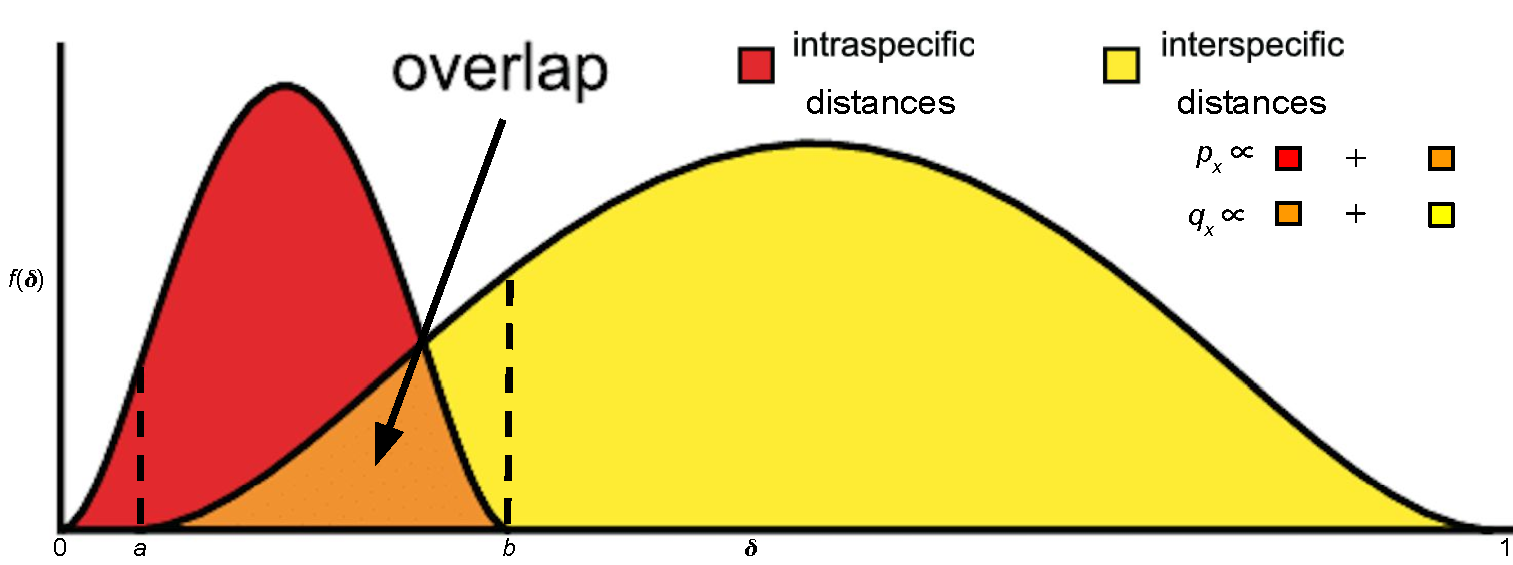
\includegraphics[width=1.0\textwidth]{Figure1}

\caption{Modified depiction from \citet{meyer2005dna} and \citet{phillips2024measure} of the overlap/separation of intraspecific and interspecific distances ($\delta$) for calculation of the DNA barcode gap metrics ($p_x$ and $q_x$) for a hypothetical species $x$. The minimum interspecific distance is denoted by $a$ and the maximum intraspecific distance is indicated by $b$. The quantity $f(\delta)$ is akin to a kernel density estimate (KDE) of the probability density function of distances. A similar visualization can be displayed for $p^{'}_x$ and $q^{'}_x$ based on intraspecific and combined interspecific distances within the interval [$a'$, $b$].}

\end{figure}

\noindent Values of the estimators obtained from Equations (1)-(4) close to or equal to zero give evidence for separation between intraspecific and interspecific distance distributions; that is, values suggest the presence of a DNA barcode gap for a target species. Conversely, values near or equal to one give evidence for distribution overlap; that is, values likely indicate the absence of a DNA barcode gap. A simple conceptual diagram to aid interpretation is shown in \textbf{Figure 2}.

\begin{figure}[H]

\centering

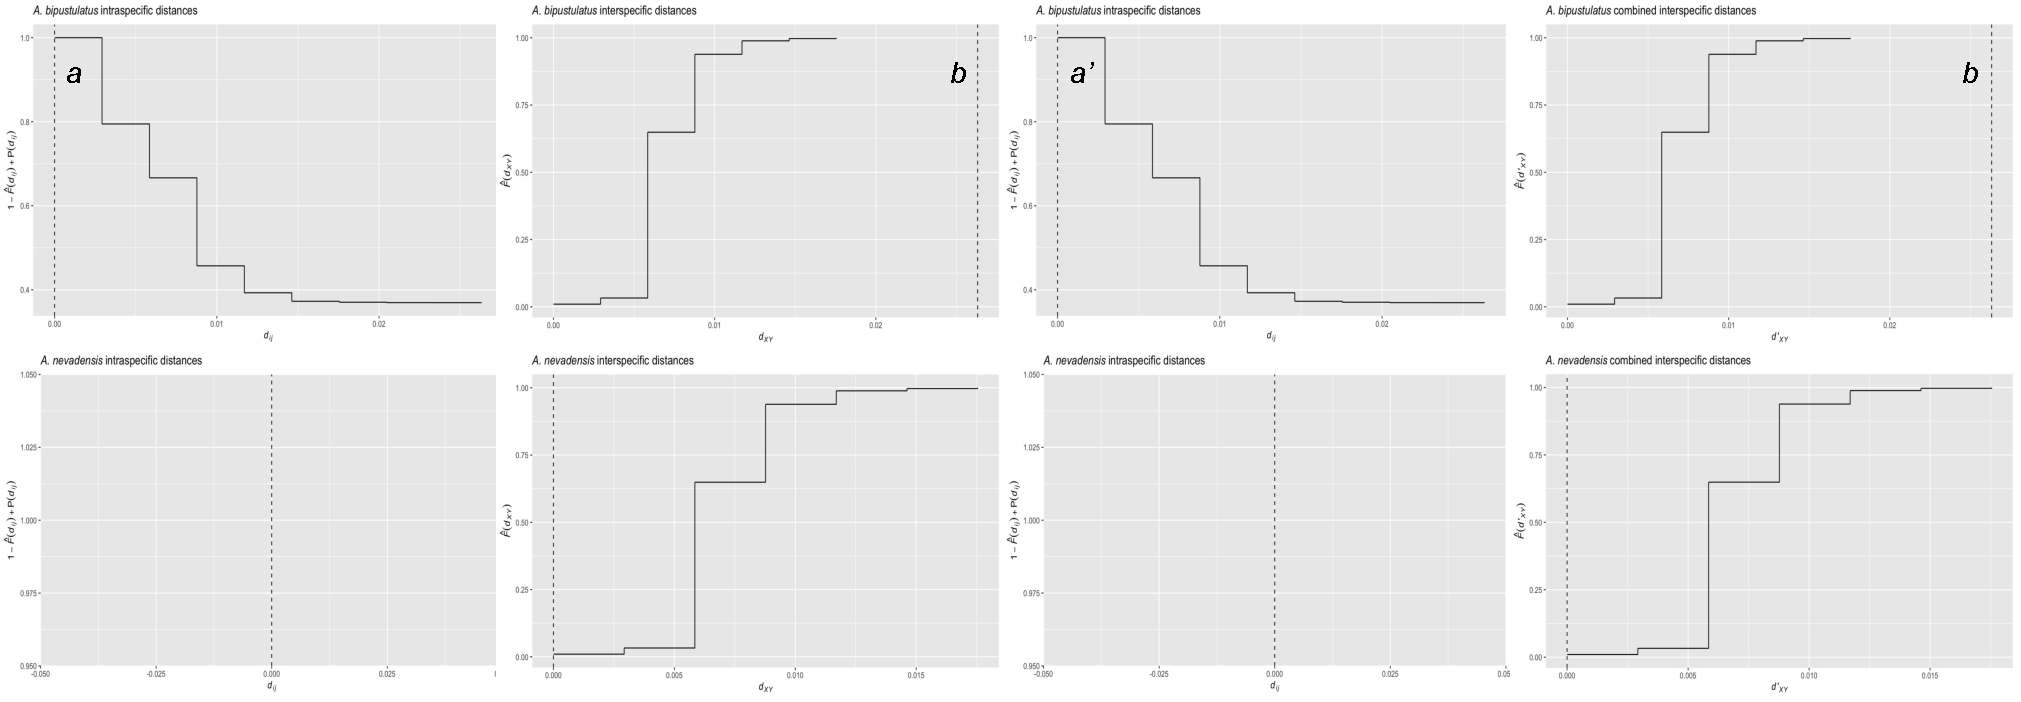
\includegraphics[width=1.0\textwidth]{Figure2}

\caption{Depiction of the DNA barcode gap metrics and their proper interpretation in cases of no overlap/complete separation and full overlap/no separation of intraspecific ($d_{ij}$) and interspecific ($d_{XY}$ and $d^{'}_{XY}$) genetic distances.}

\end{figure}

\noindent Furthermore, calculation of the DNA barcode gap estimators is convenient as they implicitly account for total distribution area within [$a$/$a'$, $b$] (including the overlap region) (\textbf{Figure 1}). 

\citeauthor{phillips2024measure}'s (\citeyear{phillips2024measure}) estimators provide a fuller picture of the interaction between intraspecific and interspecific distance distributions because they take advantage of more information when trying to quantify the DNA barcode gap. When attempting to characterize distributions of interest, most scientific studies focus solely on reporting the mean and variance. However, results can be misleading when said distributions possess identical values of these statistical summaries. The metrics of \citet{phillips2024measure} offer a deeper perspective in the same way that statistics like skewness (\textit{i.e.}, distribution asymmetry) and kurtosis (\textit{i.e.}, distribution peakedness/tailedness). It should be noted however that there is a loss of information in computing estimates of \citeauthor{phillips2024measure}'s (\citeyear{phillips2024measure}) metrics since two different sets of ($p_x$, $q_x$) and ($p^{'}_x$, $q^{'}_x$) values cause equal but distinct underlying distance distributions of $f_{\mathrm{intra}}(\delta)$ and $f_{\mathrm{inter}}(\delta)$ (\textbf{Figure 1}). In other words, under certain circumstances, the metrics cannot be determined uniquely, and so are non-identifiable in these cases. An analogy here can be made to Anscombe's quartet, a set of four datasets that differ qualitatively from one another despite having almost identical quantitative statistical summaries.  Notice that Equations (1)-(4) are simply empirical partial means of distances falling at and below, or at and exceeding, given distribution thresholds. Notice further that $a$/$a'$, and $b$ are also the first and $n$th order statistics, $X_{(1)}$ and $X_{(n)}$, respectively, with  $a$/$a' < b$,  which have been pointed out by \citet{phillips2022lack} as important for developing a statistical theory to test for the existence of the DNA barcode gap. Despite this, the underlying sampling distributions of $\eta = a - b$ and $\eta' = a' - b$ are not obvious (they involve the evaluation of convolutions). This caveat renders a formal hypothesis test cumbersome to derive since said distributions are not expected to be symmetric. The standard bootstrap resampling procedure can also fail when the estimator of interest is not well-behaved, necessitating extensions like the $m$-out-of-$n$ bootstrap discussed briefly in \citet{phillips2022lack}. This is similar to calculating bootstrap support values to assess how well tree nodes justify present data \citep{efron1996bootstrap}. However, as more data are collected, support values, along with their associated SEs, will necessarily converge to unity and zero, respectively. \citet{phillips2024measure} made an argument for the resampling of alignment sites, as opposed to distances, since DNA barcodes are short in length and sites contributing to distance distribution overlap may not be included within generated bootstrap resamples; yet, no separation could still be evident. Equations (1)-(4) can also be expressed in terms of empirical cumulative distribution functions (ECDFs) (see next section). A clear connection between the ECDF and the nonparametric MLE was noted by \citet{efron1993introduction} as well as others. However, calculated values are \textit{not} independent and identically distributed (IID) because estimated standard errors (SEs) will depend on both the number of species sampled within the genus under study, as well as the number of specimens sampled within a target species. To tease this out, \citet{phillips2024measure} suggests plotting estimator values against their estimated SEs, along with a simple random downsampling scheme. In the case of two species comprising a focal genus, one well sampled and the other poorly sampled, values of the metrics close to zero for the sufficiently sampled species will likely possess larger SEs following downsizing to match the number of poorly sampled specimens \citep{phillips2024measure}. While this scheme appears promising, challenges arise in uncertainty quantification as discussed later.

\subsection{Relationship to (Multispecies) Coalescent Theory}

The approach of \citet{phillips2024measure} differs markedly from the traditional definition of the DNA barcoding gap laid out by \citet{meyer2005dna} and \citet{meier2008use} in that the proposed metrics incorporate interspecific distances which \textit{include} the target species of interest. Furthermore, if a focal species is found to have multiple nearest neighbours, then the species possessing the smallest average distance is used \citep{phillips2024measure}. These schemes more accurately account for species' and coalescent histories inferred from contemporaneous samples of DNA sequences leading to instances of barcode sequence sharing, such as \\ interspecific hybridization/introgression events \citep{phillips2024measure}. For example, within Equations (3) and (4), the degree of distance distribution overlap/separation between a target taxon and its nearest neighbouring species, gauged from magnitudes of $p'_x$ and $q'_x$, is directly proportional to the amount of time in which the two lineages diverged from the MRCA \citep{phillips2024measure}. More specifically, $a \propto t_{XY, \hspace{1mm} \mathrm{min}}$ and $b \propto t_{ij, \hspace{1mm} \mathrm{max}}$, the minimum and maximum (unobserved) divergence time (in units of $N_e$ generations), respectively, for two different individuals ($i$, $j$) and species ($X$, $Y$) within a well-inventoried genus \citep{phillips2024measure}. Figure 1 in \citet{phillips2024measure} depicts a phylogeny for two hypothetical species, $A$ and $B$, showing paraphyly based on the sequencing of two mitochondrial loci. The (unobserved) time the two species formed, $t_{AB}$, is intermediate between $t_{XY, \hspace{1mm} \mathrm{min}}$ and $t_{ij, \hspace{1mm} \mathrm{max}}$, but theoretically, its maximum ($t_{AB, \hspace{1mm} \mathrm{max}}$) may occur more distantly in the past closer to the root comprising the MRCA for all sampled taxa (\textit{i.e.}, $t_{XY, \hspace{1mm} \mathrm{min}} < t_{AB} < t_{ij, \hspace{1mm} \mathrm{max}}$) \citep{phillips2024measure}. From a coalescence perspective, $p_x$ is the probability two lineages within species $x$ coalesce after $t_{XY, \hspace{1mm} \mathrm{min}}$, whereas $q_x$ represents the probability a lineage within species $x$ coalesces with a lineage in species $k$ (within a sample) after $t_{XY, \hspace{1mm} \mathrm{min}}$, but before $t_{ij, \hspace{1mm} \mathrm{max}}$. This approach is similar to that of \citet{desanctis2022theoretical}, who devised a coalescent model of taxonomic binning assignment accuracy given query and reference DNA sequences for two species found in a well-curated genomic database. However,  the method outlined herein is inherently simpler, easily extensible, and more intuitive, since it does not make any parametric assumptions regarding mutations along branch lengths, coalescence times, \textit{etc.} and can be applied to more than two taxa in tandem. Thus, the quantities can be used as a criterion to assess the failure of DNA barcoding in recently radiated taxonomic groups, for example, among other plausible biological explanations mentioned earlier. \textcolor{red}{Despite this, it is important to stress that while the proposed DNA barcode gap metrics and subsequent Bayesian model are biologically motivated by expectations under the multispecies coalescent, the approach is best described as coalescent-informed rather than coalescent \textit{per se} since it does not attempt to reconstruct evolutionary histories to simulate or infer coalescent processes. (See subsequent sections for further discussion.)}

\subsection{The Model}

\subsubsection{Relating the DNA Barcode Gap Metrics to the Cumulative Distribution Function}

Before delving into the derivation of the proposed DNA barcode gap metrics, review of some fundamental statistical theory is necessary. For a given random variable $X$ from a specified continuous probability distribution function (PDF), $f$, its cumulative distribution function (CDF), $F$, is defined by

\begin{align}
F_X(x) = \int_{-\infty}^{x} f(t) \,dt = \mathbb{P}(X \leq x) = 1 - \mathbb{P}(X > x). 
\end{align}

\noindent Rearranging Equation (5) gives

\begin{align}
\mathbb{P}(X > x) = 1 - F_X(x) = 1 - \mathbb{P}(X \leq x) ,
\end{align}

\noindent from which it follows that

\begin{align}
\mathbb{P}(X \geq x) = 1 - F_X(x) + \mathbb{P}(X = x).
\end{align}

\noindent Note that for a continuous $F$, $\mathbb{P}(X = x) = 0$. The CDF has many desirable statistical properties, such as boundedness, continuity, and monotonicity. 

Equations (1)-(4) can thus be written in terms of ECDFs via Equations (5) and (7) as follows, since the true underlying $F$s, are unknown \textit{a priori}, and therefore must be estimated using available sequence distance data:

\begin{align}
p_x  &= \mathbb{P}(d_{ij} \geq a) \notag \\
     &= 1 - \hat{F}_{d_{ij}}(a) + \mathbb{P}(d_{ij} = a) \\
q_x  &=  \mathbb{P}(d_{XY} \leq b) \notag \\
     &= \hat{F}_{d_{XY}}(b) \\[1ex]
p'_x &=  \mathbb{P}(d_{ij} \geq a') \notag \\
     &= 1 - \hat{F}_{d_{ij}}(a') +  \mathbb{P}(d_{ij} = a') \\
q'_x &=  \mathbb{P}(d'_{XY} \leq b) \notag \\
     &= \hat{F}_{d'_{XY}}(b).
\end{align}

\noindent Clearly from \textbf{Figure 1}, $\hat{F}_{d_{XY}}(a) = 0$ and $\hat{F}_{d_{ij}}(0)$ = 0. Similarly, $\hat{F}_{d_{ij}}(b)$ = 1 and \\ $\hat{F}_{d_{XY}}(1)$ = 1. Further, in principle, $\hat{F}_{d_{XY}}(0)$ = 0 and $\hat{F}_{d_{ij}}(1)$ = 1 when intraspecific and interspecific distributions overlap completely. Given $n$ increasing-ordered data points, the (discrete) ECDF, $\hat{F}_n(t) = \frac{1}{n}\sum_{i = 1}^n\mathds{1}_{[x_i \leq t]}$, comprises an increasing step function having jump discontinuities of size $\frac{1}{n}$ at each sample observation ($x_i$), excluding ties (or steps of weight $\frac{i}{n}$ with duplicate observations), where $\mathds{1}(x)$ is the indicator function. Note that $1 - \hat{F}_n(t)$ is the complementary ECDF (CECDF), which is a declining function. Further, $\mathbb{P}(X = t)$ is the probability that $X$ (a distance) takes on the value $t$, which is no longer necessarily zero in Equations (8)-(11) as it is within Equation (7). The ECDF/CECDF has good asymptotic behaviour in the limit of sample size: both functions are bounded on the interval [0, 1]. Equations (8)-(11) clearly demonstrate the asymmetric directionality of the proposed metrics. Plots of the ECDFs/CECDFs for nonzero intraspecific, interspecific, and combined interspecific distances, superimposed with corresponding values of $a$/$a'$ and $b$, provide a new, useful way to visualize the DNA barcode gap and \citeauthor{phillips2024measure}'s (\citeyear{phillips2024measure}) statistics. Firstly, there is no need to tune the output (\textit{e.g.}, number of bins and bin width in the case of histograms \citep{phillips2022lack}). Secondly, probabilities reflecting areas under the distance curves depicted in \textbf{Figure 1} can be directly read off the ECDF/CECDF curves. Values of the metrics can also be determined from direct inspection of the ECDF/CECDF plot by determining the corresponding $y$-value (cumulative probability) for a given value of $x$ (distance). 


\subsubsection{Integrating Frequentist and Bayesian Inference}

A major criticism of large sample (frequentist) theory is that it relies on asymptotic properties of the MLE (whose population parameter is assumed to be a fixed but unknown quantity), such as estimator normality and consistency as the sample size approaches infinity. This problem is especially pronounced in the case of binomial proportions \citep{newcombe1998confidence}. The estimated Wald SE of the sample proportion, is given by $\widehat{SE[\hat{p}}] = \sqrt{\frac{\hat{p}(1 - \hat{p})}{n}}$, where $\hat{p} = \frac{Y}{n}$ is the MLE, $Y$ is the total number of successes ($Y = \sum_{i=1}^n{y_i}$), and $n$ is the total number of trials (\textit{i.e.}, sample size). However, the above formula for the standard error is problematic for several reasons. First, it is a Normal approximation which makes use of the central limit theorem (CLT); thus, large sample sizes are required for reliable estimation. When few observations are available, SEs will be large and inaccurate, leading to low statistical power to detect a true DNA barcode gap when one actually exists. Further, resulting \textcolor{red}{confidence interval} estimates could span values less than zero or greater than one, or have zero width, which is practically meaningless. \textcolor{red}{This is the case because} when proportions are exactly equal to zero or one, resulting SEs will be exactly zero, rendering $\widehat{SE[\hat{p}}]$ given above completely useless. In the context of the proposed DNA barcode gap metrics, values obtained at the boundaries of their support are often encountered. Therefore, reliable calculation of SEs is not feasible. Given the importance of sufficient sampling of species genetic diversity for DNA barcoding initiatives, a different statistical estimation approach is necessary. 

Bayesian inference offers a natural path forward in this regard since it allows for \\ straightforward specification of prior beliefs concerning unknown model parameters and permits the seamless propagation of uncertainty, when data are lacking and sample sizes are small, through integration with the likelihood function associated with true generating processes. The posterior distribution\textcolor{red}{, $\pi(\theta | Y)$,} is given by Bayes' theorem up to a constant of proportionality, $\pi(\theta | Y) \propto \pi(Y | \theta)\pi(\theta)$, where $\theta$ are unobserved parameters, $Y$ are known data, $\pi(Y | \theta)$ is the likelihood, and $\pi(\theta)$ is the prior.  As a consequence, because parameters are treated as random variables, Bayesian models are much more flexible and generally more easily interpretable compared to frequentist approaches. Under the Bayesian paradigm, entire posterior distributions, along with their statistical summaries (\textit{e.g.}, BCIs) are outputted, rather than just long run behaviour reflected in sampling distributions, $p$-values, and CIs as in the frequentist case, thus allowing direct probability statements to be made. 

\subsubsection{Relating the DNA Barcode Gap Metrics to Mixture Models}

Essentially, from a statistical perspective, the goal herein is to nonparametrically estimate probabilities corresponding to extreme tail quantiles for positive highly skewed distributions on the unit interval  (or any closed subinterval thereof). Here, it is sought to numerically approximate the extent of proportional overlap/separation of intraspecific and interspecific distance distributions within the subinterval [$a/a'$, $b$]. This is a challenging computational problem within the current study as detailed in subsequent sections. The usual approach employs kernel density estimation (KDE), along with numerical or Monte Carlo integration of complicated PDFs, and invocation of extreme value theory (EVT) to calculate overlap (such as that for species with unusually large distances suggestive of cryptic species diversity, or deep sequence divergence due to long periods of genetic isolation); however, this requires careful selection of the bandwidth parameter, which would need to be identical for both distributions, among other considerations. This becomes problematic when fitting finite mixture models using MCMC, where nonidentifiability is rampant due to the occurrence of label switching, making clusters hard to discern across sampling iterations, and model selection challenging due to lack of exchangeability among observations \citep{stephens2000dealing}. Another problem concerns multimodality of resulting posterior distributions. For DNA barcode gap estimation, this would correspond to a two-component mixture (one for \\ intraspecific distance comparisons, and the other for interspecific comparisons), with one or more distribution modes or curve intersection points between components, and the presence of zero distance inflation. This makes parameter estimation difficult using methods like the Expectation-Maximization (EM) algorithm \citep{dempster1977maximum} as the algorithm may become stuck in suboptimal regions of the parameter search space and prematurely converge to local optima. 

The abovementioned statistical issues seem wholly plausible, especially given that the genus-level distribution of genetic distances is a mixture of closely-related (\textit{i.e.}, nearest neighbour) and more distant species. Examining \textbf{Figure 1}, depending on divergence times and other elements, interspecific distributions would be expected to comprise greater density in the centre and upper (right) tail (which make up more distantly-related taxa relative to a target species, and where there are more combinations of distance comparisons possible) compared to the lower tail overlapping with the upper (right) tail of intraspecific \\ distributions (which contain only the closest conspecifics). A key problem affecting reliable inference of the DNA barcode gap metrics is undersampling of genus-level and/or interspecific variation. An immediate, but non-trivial solution appears to be a move toward \\ next-generation DNA barcoding incorporating multiple loci \citep{collins2014known, dowton2014preliminary}. In theory, this would facilitate the detection of missing operational taxonomic units (OTUs), both extant and extinct, when attempting to better characterize a genus by capturing broader genetic variation across taxa, thereby improving species resolution that single-locus DNA barcoding might miss. Here, for simplicity, an alternate route is taken to avoid these obstacles. 

\subsubsection{Bayesian Model Setup}

Counts, $y$, of overlapping distances (as expressed in the numerator of Equations (1)-(4)) are treated as binomially distributed. Given total counts, $Y$, the likelihood is \\ $\pi(Y|\theta) = \binom{n}{Y}\theta^Y(1-\theta)^{n-Y}$, where $\binom{n}{Y}$ is the binomial coefficient expressing the number of distinct ways to choose $Y$ elements from $n$ total objects. $Y$ thus has expectation $\mathbb{E}[Y|\theta] = n\theta$, and variance $\mathbb{V}[Y|\theta] = n\theta(1 - \theta)$, where $n \in \{N, C\}$ are total counts of intraspecific and combined interspecific distances, respectively, for a target species along with its nearest neighbour species, and $n \in \{M\}$ is a total count for all interspecific species comparisons. This follows from the fact that the ECDF/CECDF is binomially distributed. The quantity thus being estimated is the parameter vector $\underaccent{\bar}{\theta} = \{p_x, q_x, p^{'}_x, q^{'}_x\}$. The metrics encompassing $\underaccent{\bar}{\theta} $ are presumed to follow a Beta($\alpha$, $\beta$) distribution, with real shape parameters $\alpha$ and $\beta$, which is a natural choice of prior on probabilities. That is,
$\pi(\theta|\alpha, \beta) = \frac{1}{\textrm{B}(\alpha, \beta)} \theta^{\alpha-1}(1-\theta)^{\beta-1}$, where $\textrm{B}(\alpha, \beta)$ is the beta function evaluated at $\alpha$ and $\beta$. The beta distribution has a prior mean of $\mathbb{E}[\theta | \alpha, \beta] = \frac{\alpha}{\alpha + \beta}$ and a prior variance equal to $\mathbb{V}[\theta | \alpha, \beta] = \frac{\alpha\beta}{(\alpha + \beta)^2(\alpha + \beta + 1)}$. In the case where $\alpha = \beta$, all generated Beta($\alpha$, $\beta$) distributions will possess the same prior expectation, whereas the prior variance will shrink as both $\alpha$ and $\beta$ increase. Such a scheme is quite convenient since the beta distribution is conjugate to the binomial distribution. Thus, the posterior distribution is also beta distributed, specifically, $\pi(\theta|Y, \alpha, \beta) = \theta^{\alpha+Y-1}(1-\theta)^{\beta+n-Y-1}$ \\ (\textit{i.e.}, Beta($\alpha + Y$, $\beta + n - Y$)), having expectation $\mathbb{E}[\theta|Y, \alpha, \beta] = \frac{\alpha + Y}{\alpha + \beta + n}$ and variance $\mathbb{V}[\theta|Y, \alpha, \beta] = \frac{(\alpha + Y)(\beta + n - Y)}{(\alpha + \beta + n)^2(\alpha + \beta + n + 1)}$. In the context of DNA barcoding, it is important that the DNA barcode gap metrics effectively differentiate between extremes of no overlap/complete separation and full overlap/no separation, corresponding to values of the metrics equal to zero and one (equivalent to total distance counts of zero and $n$), respectively. These extremes yield a posterior expectation of $\mathbb{E}[\theta|Y = 0, \alpha, \beta] = \frac{\alpha}{\alpha + \beta + n}$ and a posterior variance of $\mathbb{V}[\theta|Y = 0, \alpha, \beta] = \frac{\alpha(\beta + n)}{(\alpha + \beta + n)^2(\alpha + \beta + n + 1)}$, and $\mathbb{E}[\theta|Y = n, \alpha, \beta] = \frac{\alpha + n}{\alpha + \beta + n}$ and \\ $\mathbb{V}[\theta|Y = n, \alpha, \beta] = \frac{(\alpha + n)\beta}{(\alpha + \beta + n)^2(\alpha + \beta + n + 1)}$. Note, the posterior variances are equivalent at these thresholds for all $\alpha$ = $\beta$.

Parameters were given an uninformative Beta(1, 1) prior, which is identical to a standard uniform \textcolor{red}{, Uniform(0, 1),} prior since it places equal probability on all parameter values within its support. This distribution has an expected value of $\mu = \frac{1}{2}$ = 0.500 and a variance of $\sigma^2 = \frac{1}{12} \approx 0.083$. Further, the posterior is Beta($Y + 1$, $n - Y + 1$), from which various moments such as the expected value $\mathbb{E}[\theta|Y] = \frac{Y + 1}{n + 2}$ and variance $\mathbb{V|\theta}[Y] = \frac{(Y + 1)(n - Y + 1)}{(n + 2)^2(n + 3)}$, and other quantities, can be easily calculated. Clearly, $\mathbb{E}[\theta|Y = 0] = \frac{1}{n + 2}$ and $\mathbb{V}[\theta|Y = 0] = \frac{n + 1}{(n + 2)^2(n + 3)}$, and $\mathbb{E}[\theta|Y = n] = \frac{n + 1}{n + 2}$ and $\mathbb{V}[\theta|Y = n] = \frac{n + 1}{(n + 2)^2(n + 3)}$. For example, with a single distance \\ ($n$ = 1) for a given species (wherein two specimens are compared), and where the distance is not overlapping, on average, $\theta$ will be equal to $\mu = \frac{1}{3}$ = 0.333, with a variance of \\ $\sigma^2 = \frac{2}{36} = \frac{1}{18} \approx$ 0.056. In contrast, with $n$ = 100 individuals and there is no overlap, the mean reduces to $\mu = \frac{1}{102} \approx$ 0.010, with a variance of $\sigma^2 = \frac{101}{1071612}$ = 9.425$\hspace{1mm} \times \hspace{1mm} 10^{-5}$. When \\ $n$ = 1 and there is overlap, the mean is $\mu = \frac{2}{3}$ = 0.667, having a variance of $\sigma^2 \approx$ 0.056. For \\ $n$ = 100 where all distances overlap, $\theta$ has expectation $\mu = \frac{101}{102} \approx$ 0.990 and variance \\ $\sigma^2 \approx$ 9.425$\hspace{1mm} \times \hspace{1mm} 10^{-5}$. These edge case examples have good asymptotic behaviour with \\ increasing sample size (variance tends to zero), and demonstrate that the Beta(1, 1) \\ distribution serves as a reasonable first-pass prior for DNA barcode gap estimation using \citeauthor{phillips2024measure}'s (\citeyear{phillips2024measure}) metrics, though tighter bounds can be achieved through increasing both $\alpha$ and $\beta$. In general however, when possible, it is always advisable to incorporate prior information, even if only weak, rather than simply imposing complete ignorance in the form of a flat prior distribution. In the case of unimodal distributions, the (estimated) posterior mean often possesses the property that it readily decomposes into a convex linear combination, in the form of a weighted sum, of the (estimated) prior mean and the MLE. That is $\hat{\mu}_\mathrm{posterior} = w\hat{\mu}_\mathrm{prior} + (1-w)\hat{\mu}_\mathrm{MLE}$, where, for the beta distribution, $w = \frac{\alpha + \beta}{\alpha + \beta + n}$, and $\hat{\mu}_\mathrm{prior}$, along with $\hat{\mu}_\mathrm{MLE}$ are given in the preceding sections. Therefore, with sufficient data, $w \rightarrow 0$ as $n \rightarrow \infty$, regardless of the values of $\alpha$ and $\beta$, and the choice of prior distribution becomes less important since the posterior will be dominated by the likelihood. For the Beta(1, 1), $w = \frac{2}{2 + n}$, with $n$ = 1 giving $w = \frac{2}{3}$ = 0.667. For $n$ = 100, the prior weight becomes $w = \frac{2}{102} \approx$ 0.020. The full Bayesian model for species $x$ is thus given by

\begin{align}
\notag y_\mathrm{lwr} &\sim \mathrm{Binomial}(N, p_\mathrm{lwr}) \\ 
\notag y_\mathrm{upr} &\sim \mathrm{Binomial}(M, p_\mathrm{upr}) \\ 
y^{'}_\mathrm{lwr} &\sim \mathrm{Binomial}(N, p^{'}_\mathrm{lwr}) \\ 
 \notag y^{'}_\mathrm{upr} &\sim \mathrm{Binomial}(C, p^{'}_\mathrm{upr}) \\ 
\notag p_\mathrm{lwr}, p_\mathrm{upr}, p^{'}_\mathrm{lwr}, p^{'}_\mathrm{upr}
&\sim \mathrm{Beta}(1, 1)
\end{align}

\noindent Note that $p_x$, $q_x$, $p^{'}_x$, and $q^{'}_x$ in Equations (1)-(4) are denoted $p_\mathrm{lwr}$, $p_\mathrm{upr}$, $p^{'}_\mathrm{lwr}$, and $q^{'}_\mathrm{upr}$, respectively within Equation (12) for easy distinction between MLEs and Bayesian posterior estimates. Further, $y_\mathrm{lwr}$, $y_\mathrm{upr}$, $y^{'}_\mathrm{lwr}$, and $y^{'}_\mathrm{upr}$ are calculated from the numerators of Equations (1)-(4), respectively. The above statistical theory and derivations lay a good foundation for the remainder of this paper.

\subsubsection{Computational Details}

The proposed model is inherently vectorized to allow processing of multiple \\ species/marker datasets simultaneously. Model fitting was achieved using the Stan \\ probabilistic programming language \citep{carpenter2017stan} framework for Hamiltonian Monte Carlo (HMC) \citep{neal2011mcmc} via the No-U-Turn Sampler (NUTS) sampling algorithm \citep{hoffman2014no} through the {\tt rstan} R package (version 2.32.6) \\ \citep{stan2023rstan} in R (version 4.4.1) \citep{rcore2024language}. Four Markov chains were run for 2000 iterations each in parallel across four cores with random parameter initializations. Within each chain, a total of 1000 samples was discarded as warmup (\textit{i.e.}, burnin) to reduce dependence on starting conditions and to ensure posterior samples are reflective of the equilibrium distribution. Further, 1000 post-warmup draws were utilized per chain during the sampling phase. Because HMC/NUTS results in dependent samples that are minimally autocorrelated, chain thinning is not required. Each of these tuning parameters \textcolor{red}{(\textit{i.e.}, the number of chains, the number of iterations, and the number of burnin/warmup samples)} reflect default MCMC settings in Stan to control both bias and variance, \\ respectively, in the resulting draws. All analyses in the present work were carried out on a 2023 Apple MacBook Pro with M2 chip and 16 GB RAM running macOS Ventura 13.2. A random seed was set to ensure reproducibility of model results. Outputted estimates were rounded to three decimal places of precision. Posterior draws and posterior distributions of the metrics were visualized as scatterplots and KDE plots, respectively, using the {\tt ggplot()} function within the {\tt ggplot2} R package (version 3.5.1) \citep{wickham2016ggplot2} with the default Gaussian kernel and optimal smoothness selection. To successfully run the Stan program, end users must have installed an appropriate compiler (such as GCC or Clang) which is compatible with their operating system, such as macOS.

Convergence was assessed both visually and quantitatively as follows: (1) through \\ examining parameter traceplots, which depict the trajectory of accepted MCMC draws as a function of the number of iterations, (2) through monitoring the Gelman-Rubin potential scale reduction factor statistic   ($\hat{R}$)  \citep{gelman1992iterative, vehtari2017rank}, which measures the concordance of within-chain \textit{versus} between-chain variance, and (3) through calculating the effective sample size (ESS) for each parameter, which quantifies the number of independent samples generated Markov chains are equivalent to. Mixing of chains was deemed sufficient when traceplots looked like ``fuzzy caterpillars", $\hat{R} < 1.01$, and effective sample sizes were reasonably large \citep{gelman2020bayesian}.
After sampling, a number of summary quantities were reported, including posterior means, posterior SDs, and posterior quantiles from which 95\% BCIs could be computed to make probabilistic inferences concerning true population parameters. To validate the overall correctness of the proposed statistical model given by Equation (12), as a means of comparison, posterior predictive checks (PPCs) were also employed to generate binomial random variates in the form of mean counts from the posterior predictive distribution; that is $\underaccent{\bar}{\gamma} = \{Np_x, Mq_x, Np^{'}_x, Cq^{'}_x\}$, to verify that the model adequately captures relevant features of the observed data. It needs to be mentioned that the Bayesian framework outlined herein mirrors the traditional task of parameter inference seen in the statistical literature. This is in contrast to what is usually done in species delimitation studies employing BEAST for example, wherein often millions of iterations are necessary to reach convergence since BEAST jointly infers phylogenetic relationships existing among sampled DNA sequences. \textcolor{red}{Note that a full Bayesian phylogenetic analysis could take days/weeks to run depending on dataset size (\textit{i.e.}, the number of species and taxon DNA sequences). Thus, the only things lost are time (both actual and computational) and human effort necessary for tree generation and parameter estimation; accuracy of results would not likely be affected.} As phylogenetic reconstruction is a computationally complex task whose solution becomes less tractable as the number of taxa and/or the DNA sequences grows, it generally cannot be solved in polynomial time (\textit{i.e.}, it is NP-complete).

\subsubsection{Probabilistic Interpretation of the DNA Barcode Gap Metrics}

The proposed Bayesian model outlined here has a straightforward interpretation (\textbf{Table 1}). 

\begin{table}[H]
    \centering
    \small
    \caption{Interpretation of the DNA barcode gap estimators within [$a/a'$, $b$]}.
    \label{tab:parameters}
    \begin{tabular}{cp{0.7\linewidth}}
    \hline
    \textbf{Parameter} & \textbf{Explanation} \\
    \hline
    $p_x$/$p_{\text{lwr}}$ & When $p_x/p_{\text{lwr}}$ is close to 0 (1), it suggests that the probability of intraspecific (interspecific) distances being larger (smaller) than interspecific (intraspecific) distances is low (high) on average, while the probability of interspecific (intraspecific) distances being larger (smaller)  than intraspecific (interspecific) distances is high (low) on average; that is, there is (no) evidence for a DNA barcode gap.\\
        & \\[-2mm]
     $q_x$/$p_{\text{upr}}$ & When $q_x/p_{\text{upr}}$ is close to 0 (1), it suggests that the probability of interspecific (intraspecific) distances being larger (smaller) than intraspecific (interspecific) distances is high (low) on average, while the probability of intraspecific (interspecific) distances being larger (smaller) than interspecific (intraspecific) distances is low (high) on average; that is, there is (no) evidence for a DNA barcode gap. \\
        & \\[-2mm]
    $p^{'}_x$/$p^{'}_{\text{lwr}}$ & When $p^{'}_x/p^{'}_{\text{lwr}}$ is close to 0 (1), it suggests that the probability of intraspecific (combined interspecific distances for a target species and its nearest neighbour species) distances being larger (smaller) than combined interspecific distances for a target species and its nearest neighbour species (intraspecific distances) is low (high) on average, while the probability of combined interspecific distances for a target species and its nearest neighbour species (intraspecific distances) being larger (smaller) than intraspecific distances (combined interspecific distances for a target species and its nearest neighbour species) is high (low) on average; that is, there is (no) evidence for a DNA barcode gap.\\
        & \\[-2mm]
     $q^{'}_x$/$p^{'}_{\text{upr}}$ & When $q^{'}_x/p^{'}_{\text{upr}}$ is close to 0 (1), it suggests that the probability of combined interspecific distances for a target species and its nearest neighbour species (intraspecific distances) being larger (smaller) than intraspecific distances (combined interspecific distances for a target species and its nearest neighbour species) is high (low) on average, while the probability of intraspecific distances (combined interspecific distances for a target species and its nearest neighbour species) being larger (smaller) than combined interspecific distances for a target species and its nearest neighbour species (intraspecific distances) is low (high) on average; that is, there is (no) evidence for a DNA barcode gap.\\
    \hline
    \end{tabular}
\end{table}

\subsection{\textit{Agabus} Case Study}

The DNA barcode gap statistics have been shown to hold strong promise for reliable DNA barcode gap detection when applied to the predatory diving beetles \textit{Agabus} (Coleoptera: Dytiscidae) \citep{phillips2024measure}. With a Holarctic range, despite their ease of sampling and well-established taxonomy, this group possesses few morphologically-distinct taxonomic characters that readily facilitate their assignment to the species level \citep{bergsten2012effect}. Accurate taxon discrimination within \textit{Agabus} is paramount since several species are currently classified as endangered on the International Union for Conservation of Nature (IUCN) Red List (\href{https://www.iucnredlist.org}{https://www.iucnredlist.org}) due to habitat fragmentation/loss, water pollution, and climate change. Further, the proposed metrics indicate that sister species pairs from this taxon are often difficult to distinguish on the basis of their DNA barcode sequences \citep{phillips2024measure}, which may be caused by \textit{Agabus}' increased degree of non-monophyly at wider geospatial scales, occurrence of hybridization/introgression, or presence of synonymy \citep{bergsten2012effect}. \textcolor{red}{DNA barcoding data are inherently ``messy" and the use of \textit{Agabus} by \citet{phillips2024measure} was chosen precisely to illustrate the challenges of employing single-locus genetic markers for specimen identification and species delimitation.} Using sequence data from three mitochondrial cytochrome markers (5'-COI, 3'-COI, and cytochrome $b$ (CYTB)) obtained from BOLD and GenBank, results from \citet{phillips2024measure} highlight that DNA barcoding has been a one-sided argument. For instance, DNA barcode libraries are strongly skewed towards mitochondrial marker variation like that seen in COI, in addition to \\ over-emphasizing certain taxonomic groups (\textit{e.g.}, Lepidoptera) and geographic regions (\textit{e.g.}, Costa Rica). As a result of DNA barcoding's ``easy" targeting approach, this has led to a false sense of certainty in the form of taxon ``blindspots", particularly for poorly-understood taxonomic groups exhibiting interesting eco-evolutionary dynamics, such as Canadian \\ freshwater fishes \citep{hubert2008identifying, morey2024taxonomic} and North American freshwater fishes more broadly \citep{april2011genetic}. \citeauthor{phillips2024measure}'s (\citeyear{phillips2024measure}) findings point to the need to balance both the sufficient collection of specimens, as well as the extensive sampling of species when populating DNA barcode reference libraries with high fidelity taxon records. This is an important problem to resolve since, while DNA barcoding's use as identification tool is widely accepted, its promise for species demarcation, is much more hotly debated. Not surprisingly, DNA barcode libraries for most taxonomic groups are biased toward the collection of as many different species as possible \citep{phillips2015exploration, phillips2019incomplete, phillips2022lack}. The newly outlined DNA barcode gap metrics provide a useful numeric summary of the overall performance and relability of DNA barcoding and attempts to narrow the divide between specimen identification and species discovery using single-locus molecular data.

\subsection{\textcolor{red}{5'-COI and 3'-COI Datasets}}

\textcolor{red}{Briefly, using the R package {\tt MACER} \citep{young2021macer}, DNA sequences were downloaded from GenBank and BOLD and processed using a stringent workflow to obtain two 600-bp high-quality FASTA alignment for 5'-COI and 3'-COI representing 531 and 1375 species, and comprising 190 and 212 unique haplotypes, respectively. The resulting alignments contained no stop codons, ambiguous nucleotides, or other problematic artifacts that bias genetic diversity estimates. Further, both species- and genus-level distance outliers were excluded based on the interquartile range (\textit{i.e.}, 1.5$\times$IQR rule) \citep{young2021macer}. Genetic distances were calculated using uncorrected p-distances. Note, DNA barcode gap estimation is only possible for species having at least two specimen records because only one distance can be calculated.}

\subsection{\textcolor{red}{CYTB Dataset}}

The \textit{Agabus} CYTB dataset analyzed by \citet{phillips2024measure} is \textcolor{red}{also} revisited herein for the species \textit{A. bipustulatus} and \textit{A. nevadensis}, since these taxa were the sole representatives for this locus, with the most and the least specimen records, respectively ($N$ = 701 and \\ $N$ = 2) across all three assessed molecular markers. \textcolor{red}{Interestingly, new evidence \citep{pallares2024genomic} points to \textit{A bipustulatus} and \textit{A nevadensis} encompassing a tight species complex, with the latter species being deeply nested within the former. From a DNA barcoding standpoint, this suggests that these two beetle species are effectively identical. \textit{A nevadensis} is a narrow-ranging endemic alpine ecotype of \textit{A bipustulatus} found within the Sierra Nevada mountain range on the Iberian Peninsula (Spain) likely arising from an incipient speciation process with substantial recent introgression \citep{pallares2024genomic}. \textit{A. bipustulatus} and \textit{A. nevadensis} are not the typical clean and well-delimited sister species pair expected when demonstrating the utility of a newly proposed statistical method, but is noteworthy for other reasons.} \textcolor{red}{Data preparation was identical to that of COI, resulting in a high-quality 342-bp sequence alignment.} Outliers were only present for \textit{A. bispustulatus}: 21 at the genus level and a further three at the species level. These excluded records could reflect either taxon misidentifications or potential cryptic species diversity. To verify this, dimension reduction techniques like Principal Component Analysis (PCA) should be employed to ascertain \\ whether filtered records form distinct clusters. \textit{A. bipustulatus} comprised 45 total haplotypes, whereas \textit{A. nevadensis} possessed only one haplotype. This dataset is a prime illustrative example highlighting the issue of inadequate taxon sampling, which arises frequently in large-scale phylogenetic and phylogeographic studies, in several respects. First, from a statistical viewpoint, sample sizes reflect extremes in reliable parameter estimation. Second, from a DNA barcoding perspective, \textit{Agabus} currently comprises about 200 extant Linnean species according to the Global Biodiversity Information Facility (GBIF) \\ (https://www.gbif.org); yet, due to the level of convenience sampling inherent in taxonomic collection efforts for this genus, adequate representation of species and genetic diversity is far from complete. Indeed, herein, species coverage for CYTB is only around 1.000\%. Not surprisingly, CYTB performed poorly as a DNA barcode locus for \textit{Agabus} despite having the highest specimen representativeness for a given species ($N = 701$, \textit{A. bipustulatus}) and displaying good separation of genetic sequences among all three mitochondrial genes examined in \citeauthor{phillips2024measure}'s (\citeyear{phillips2024measure}) study; yet no DNA barcode gap was observed since all metrics were found to be equal to 1.000 for this species. The situation for \textit{A. nevadensis} is much less clear ($p_x$ = $p^{'}_x$ = 1, $q_x$ = $q^{'}_x$ = 0.010). (See Figure 3 in \citet{phillips2024measure}.) This finding strongly reinforces how low sample sizes can lead to incorrect interpretation of the DNA barcode gap \textcolor{red}{and may even provide credence to conclusions reached by \citet{pallares2024genomic}}.

\section{Results and Discussion}

\textcolor{red}{Results of the Bayesian coalescent-informed model outlined herein for all molecular gene loci and \textit{Agabus} species can be reproduced entirely using the R script provided within the \textbf{Data Accessibility Statements} accompanying this paper. The included ``point-and-click" script will automatically generate and save all required data output and visualizations locally to a user's working directory. Furthermore, the program is easily extended to other molecular markers and taxa.}

\subsection{\textcolor{red}{CYTB Dataset}}

ECDF/CECDF plots were generated using the base R function {\tt ecdf()}, along with {\tt ggplot()}, and are displayed in \textbf{Figure 3}. Interpretation is simple: in the case of \\ \textit{A. bipustulatus}, for both $p_x$ and $p^{'}_x$, all distances are greater than $a$ = 0, with 36.900\% of distances equal to $a/a'$. Conversely, both $q_x$ and $q^{'}_x$ equal one because all interspecific distances are less than $b \approx$ 0.026; for \textit{A. nevadensis}, both $q_x$ and $q^{'}_x$ are approximately equal to 0.010 since only about 1\% of distances fall below $b$ = 0. In the case of $p_x$ and $p^{'}_x$, both statistics equal 1.000 since all distances were found to be zero.

\begin{figure}[H]

\centering

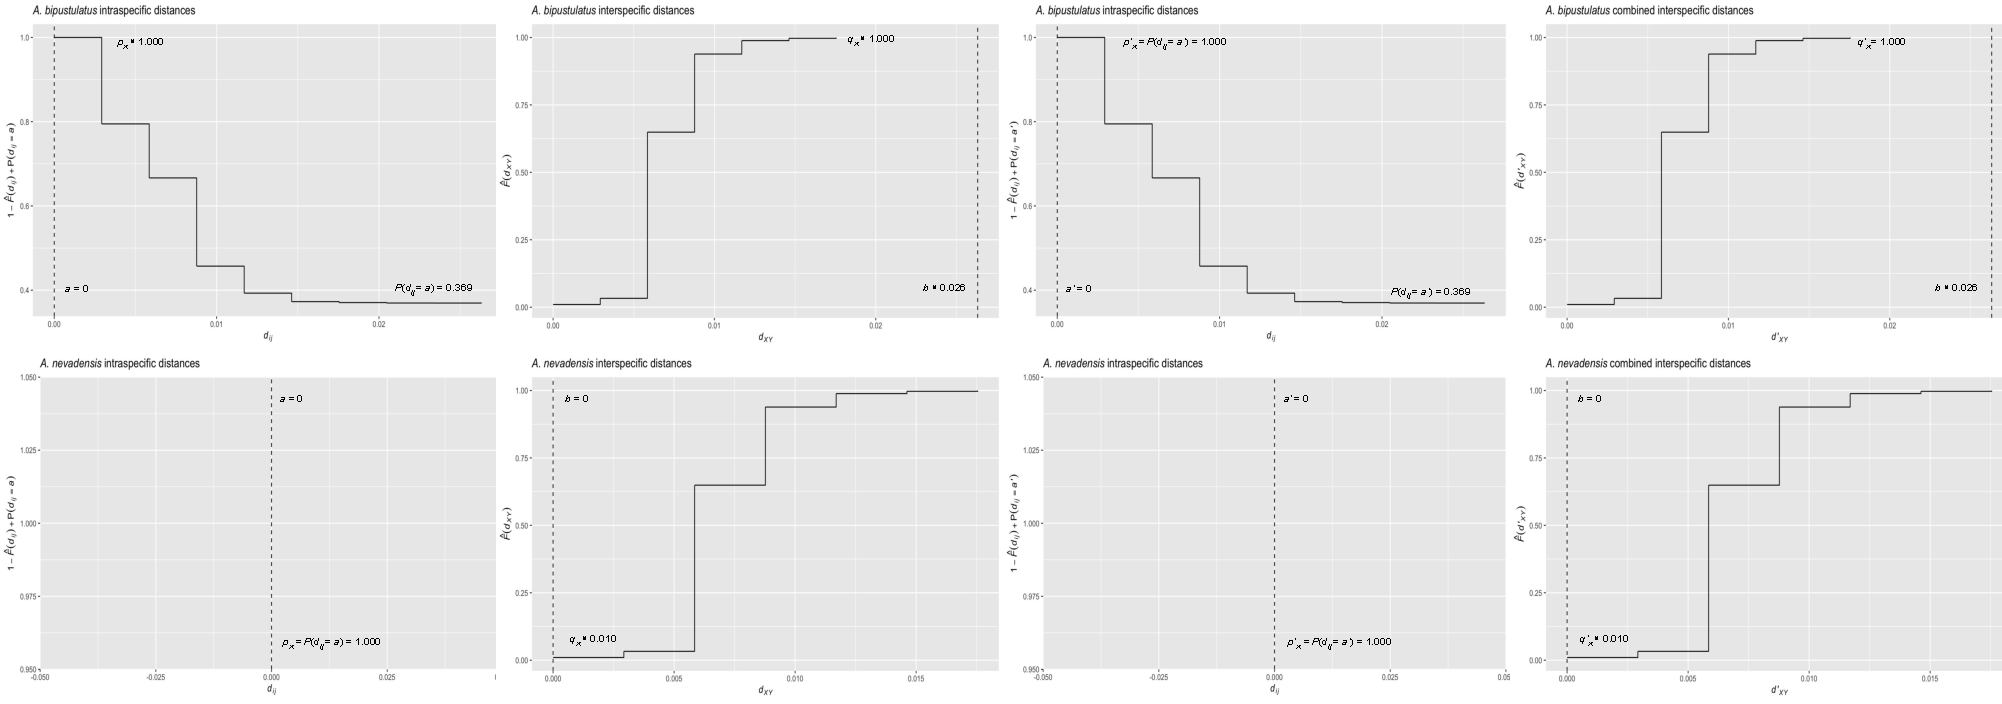
\includegraphics[width = 1.0\textwidth]{Figure3}

\caption{ECDF/CECDF plots of the DNA barcode gap metrics for \textit{A. bipustulatus} and \textit{A. nevadensis} with $a$/$a'$ and $b$ clearly indicated as dashed vertical lines. When all genetic distances are equal to zero, no step function is shown.}

\end{figure}

\noindent MCMC parameter traceplots showed rapid mixing of chains to the stationary distribution (\textcolor{red}{\textbf{Supplementary Figure 1}}). Further, all $\hat{R}$ and ESS values (both not shown) were close to their recommended cutoffs of one and thousands of samples, respectively, indicating chains are both well-mixed and have converged to the posterior distribution. Bayesian posterior estimates were reported alongside frequentist MLEs, in addition to SEs, posterior SDs, 95\% CIs, and 95\% BCIs (\textbf{Table 2}).


\begin{table}[H]

\small

\centering

\caption{Nonparametric frequentist and Bayesian estimates of distance distribution overlap/separation for the DNA barcode gap coalescent model parameters applied to \textit{A. bipustulatus} ($N$ = 701) and \textit{A. nevadensis} ($N$ = 2) for CYTB, including 95\%  CIs and BCIs. BCIs are based on 4000 posterior draws. All parameter estimates are reported to three decimal places of precision.}


\begin{tabular}{cccc} \hline

\textbf{Species} & \textbf{Parameter} & \textbf{MLE (SE, 95\% CI)} & \textbf{Bayes Est. (SD; 95\% BCI)} \\  \hline
\textit{A. bipustulatus} & $p_x/p_\mathrm{lwr}$ & 1.000 (0.000; 1.000-1.000) & 1.000 (0.000; 1.000-1.000) \\
\textit{A. bipustulatus} & $q_x/p_\mathrm{upr}$ & 1.000 (0.000; 1.000-1.000) & 1.000 (0.000; 0.999-1.000) \\
\textit{A. bipustulatus} & $p^{'}_x/p^{'}_\mathrm{lwr}$ & 1.000 (0.000; 1.000-1.000) & 1.000 (0.000; 1.000-1.000)  \\
\textit{A. bipustulatus} & $q^{'}_x/p^{'}_\mathrm{upr}$ & 1.000 (0.000; 1.000-1.000) & 1.000 (0.000; 0.999-1.000) \\


\textit{A. nevadensis} & $p_x/p_\mathrm{lwr}$ & 1.000 (0.000; 1.000-1.000) & 0.835 (0.144; 0.470-0.996) \\
\textit{A. nevadensis} & $q_x/p_\mathrm{upr}$ & 0.010 (0.002; 0.006-0.014) & 0.010 (0.002; 0.007-0.014) \\
\textit{A. nevadensis} &  $p^{'}_x/p^{'}_\mathrm{lwr}$ & 1.000 (0.000; 1.000-1.000) & 0.834 (0.138; 0.481-0.994) \\
\textit{A. nevadensis} &  $q^{'}_x/p^{'}_\mathrm{upr}$ & 0.010 (0.070; -0.128-0.148) & 0.010 (0.002; 0.007-0.014) \\


\hline


\end{tabular}

\end{table}

\noindent  CIs were calculated using the usual large sample  $(1-\alpha)100\%$-level interval estimate given by $\hat{p} \hspace{1mm} \pm z_{1 - \frac{\alpha}{2}}\sqrt{\frac{\hat{p}(1 - \hat{p})}{n}}$, where $z_{1 - \frac{\alpha}{2}}$ = 1.960 is the critical value for 95\% confidence \\ (\textit{i.e.}, the 97.5th percent quantile from the standard Normal distribution), and $\alpha$ is the stated significance level (here, 5\%). Given a ($1 - \alpha$)100\% CI, with repeated sampling, on average ($1 - \alpha$)100\% of constructed intervals will contain the true parameter of interest, assuming a correctly-specified statistical model; on the other hand, any given CI will either capture or exclude the true parameter with 100\% certainty. This in stark contrast to a BCI, where the true parameter is contained within said interval with ($1 - \alpha$)100\% probability, contingent on the data generating model being correct. Note, by default Stan computes equal-tailed (central) BCIs such that there is equal area situated in the left and right tail of the posterior distribution. For a 95\% BCI, this corresponds to the 2.5th and 97.5th percent quantiles. However, constructed intervals are usually only valid for symmetric or nearly symmetric distributions. Given the bounded nature of the DNA barcode gap metrics, whose posterior distributions, as expected, show considerable skewness, an alternative approach to reporting BCIs, such as Highest Posterior Density (HPD) intervals \citep{chen1999monte} or shortest probability intervals (SPIn) \citep{liu2015simulation} is warranted. Although the data for \textit{Agabus} were not found to be consistent with a value of zero for the metrics (suggesting the existence of a DNA barcode gap) for either species, this is clearly a case that must differentiated from one where some or all of the estimators attain a value of one (indicating no DNA barcode gap likely exists).  As such asymmetric intervals generally attain greater statistical efficiency (in the form of smaller mean squared error (MSE) or variance) and higher coverage probabilities than more standard interval estimates, careful in-depth comparison is left for future work. 

Findings based on nonparametric MLEs and Bayesian posterior means were quite \\ comparable with one another and show evidence of complete overlap in intraspecific, \\ interspecific, and combined interspecific distances for \textit{A. bipustulatus} in both the \\ $p$/$q$/$p_{\mathrm{lwr}}$/$p_{\mathrm{upr}}$ and $p'$/$q'$/$p^{'}_{\mathrm{lwr}}$/$p^{'}_{\mathrm{upr}}$ directions since the metrics and their intervals attain \\ magnitudes very close or equal to one, with minimal noise (\textbf{Table 2}). As a result, this likely indicates that no DNA barcode gap is present for this species. Such findings are strongly reinforced by the very tight clustering of posterior draws (\textbf{Figure 4}) and associated interval estimates owing to the large number of specimens sampled for this species.

\begin{figure}[H]

\centering

\small

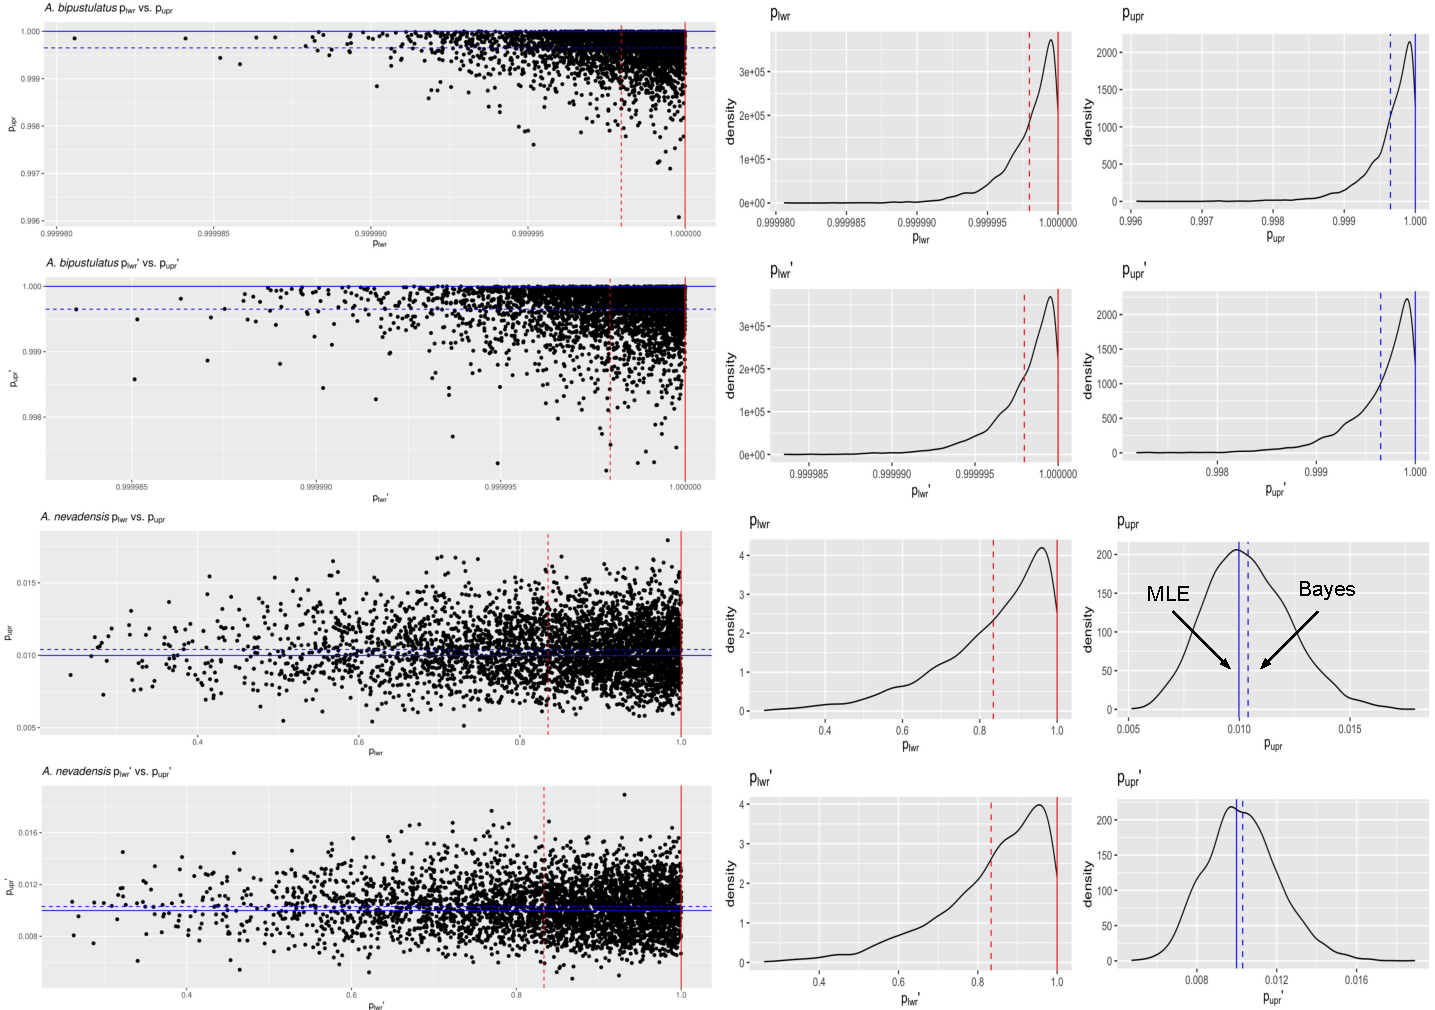
\includegraphics[width=0.80\textwidth]{Figure5}

\caption{Scatterplots (black solid points) and distributions (black solid lines) depicting the DNA barcode gap metrics for \textit{A. bipustulatus} ($N$ = 701) and  \textit{A. nevadensis} ($N$ = 2) across CYTB based on 4000 Bayesian posterior draws. MLEs and posterior means are displayed as coloured (red/blue) solid and dashed lines for the metrics, respectively.}

\end{figure}

\noindent On the other hand, the situation for \textit{A. nevadensis} is more nuanced, as posterior values are further spread out (\textbf{Table 2} and \textbf{Figure 4}), suggesting less overall certainty in true parameter values given the low specimen sampling coverage for this taxon. Of note, calculated SEs and SDs are large, with the 95\% CIs and 95\% BCIs being quite wide in most cases, consistent with much uncertainty regarding the computed frequentist and Bayesian posterior means of the DNA barcode gap metrics. For instance, the Bayesian analysis suggests that the data are consistent with both $p_{\mathrm{lwr}}$ and $p^{'}_{\mathrm{lwr}}$ ranging from approximately 0.500-1.000 due to the large SD of about 0.140. The posterior means associated with these estimates themselves are also far from one. The BCI for $p_{\mathrm{upr}}$ and $p^{'}_{\mathrm{upr}}$ also spans an order of magnitude, with the lower tail estimate of 0.007 being very close to zero. Further, regarding the frequentist analysis for the same species, the 95\% CI for $q_x$ is quite wide, reflecting considerable uncertainty in its true parameter value. Similarly, that for $q^{'}_x$ extends to negative values at the left endpoint, due to the corresponding SE of 0.070 being too high as a result of the extremely low sample size of $n$ = 2 individuals sampled (\textbf{Table 2}). Since the 95\% CI for $q^{'}_x$ truncated at the lower endpoint includes the value of zero, the null hypothesis for the presence of a DNA barcode gap would not be rejected. Despite this, it is worth noting that truncation is not standard statistical practice and will likely lead to an interval with less than 95\% nominal coverage having high relative error. In such cases, more appropriate confidence interval methods like the Wilson score interval, the exact (Clopper-Pearson) interval, or the Agresti-Coull interval should be employed \citep{newcombe1998confidence, agresti1998approximate}. KDEs for \textit{A. bipustulatus} are strongly left (negatively) skewed (\textbf{Figure 4}), whereas those for \textit{A. nevadensis} exhibit more symmetry, especially for $p_{\mathrm{upr}}$ and $p^{'}_{\mathrm{upr}}$ (\textbf{Figure 4}). These differences are likely due to the stark contrast in sample sizes for the two examined species. Nevertheless, simulated counts of overlapping specimen records from the posterior predictive distribution \textcolor{red}{(\textbf{Supplementary Table 1})} were found to be very close to observed counts for both species, indicating that the proposed model adequately captures underlying variation. Despite this, while BCIs were found to be narrow for \textit{A. bipustulatus}, they were quite wide for \textit{A. nevadensis} (particularly for $y_{\mathrm{upr}}$ and $y^{'}_{\mathrm{upr}}$), suggesting that further model improvements could be made. Obtained results suggest that use of the Beta(1, 1) prior may not be appropriate given a low number of collected individuals for most taxa in DNA barcoding efforts. This suggests that further consideration of more informative beta priors is worthwhile. This is clear for \textit{A. nevadensis}, where use of a stronger prior will likely eliminate the issue regarding accurate estimation of $p_{\mathrm{lwr}}$ and $p^{'}_{\mathrm{lwr}}$ and stabilize their uncertainty.

\section{\textcolor{red}{5'-COI and 3'-COI Datasets}}

\section{Conclusion}

Herein, the accuracy of the DNA barcode gap was analyzed from a rigorous statistical lens to expedite both the curation and growth of reference sequence libraries, ensuring they are populated with high quality, statistically defensible specimen records fit for purpose to address standing questions in ecology, evolutionary biology, biodiversity forensics, \\ conservation, management, and restoration. To accomplish this, recently proposed, easy to calculate, nonparametric MLEs were formally derived using ECDFs/CECDFs and applied to assess the extent of overlap/separation of distance distributions within and among two species of predatory water beetles in the genus \textit{Agabus} sequenced at CYTB using a Bayesian binomial count model with conjugate beta priors. Findings highlight a high level of parameter uncertainty for \textit{A. nevadensis}, whereas posterior estimates of the DNA barcode gap metrics for \textit{A. bipustulatus} are much more certain. \textcolor{red}{This result may further support the recent finding by \citet{pallares2024genomic} that these two taxa are indistiguishable based on their DNA barcodes and form a species complex, but only once further sampling is conducted for \textit{A. nevadensis}.} Based on these results, it is imperative that specimen sampling be prioritized to better reflect actual species boundaries. More generally, apart from the metrics being employed to better highlight the importance of within-species genetic diversity versus between-species divergence, it is expected that the approach developed herein will be of broad utility in applied fields, such as DNA-based detection of seafood fraud within global supply chains, and in the determination of species occupancy/detection probabilities at ecological sites of interest using active and passive environmental DNA (eDNA) methods such as metabarcoding.

Since the DNA barcode gap metrics often attain values very close to zero (suggesting no overlap and complete separation of distance distributions) and/or very near one (indicating no separation and complete overlap), in addition to more intermediate values, a noninformative Beta($\frac{1}{2}, \frac{1}{2}$) prior may be more appropriate over complete ignorance imposed by a Beta(1, 1) prior. The former distribution is U-shaped symmetric and places greater probability density at the extremes of the distribution due to its heavier tails, while still allowing for variability in parameter estimates within intermediate values along its domain. This feature is appealing since \citeauthor{phillips2024measure}'s (\citeyear{phillips2024measure}) metrics often take on values of zero and one. Note that this prior is Jeffreys' prior density \citep{jeffreys1946invariant}, which is  proportional to the square root of the Fisher information $\mathcal{I}(\theta)$; that is,
$\pi(\theta) \propto \theta^{-\frac{1}{2}}(1-\theta)^{-\frac{1}{2}}$. Jeffreys' prior has several desirable statistical  properties as a prior: that it is inversely proportional to the standard deviation of the binomial distribution, and most notably, that it is invariant to model reparameterization \citep{gelman2014bayesian}. However, this prior can lead to divergent transitions, among other problems, imposed by complex geometry (\textit{i.e.}, curvature) in the posterior space since many iterative stochastic MCMC sampling algorithms experience difficulties when exploring high density distribution regions. Thus, remedies to resolve them, such as lowering the step size of the HMC/NUTS sampler, should be attempted in future work, along with other approaches such as empirical Bayes estimation to approximate beta prior hyperparameters from observed data through the MLE or other methods of parameter estimation, such as the method of moments. Alternatively, hierarchical modelling could be employed to estimate separate distribution model hyperparameters for each species and/or compute distinct estimates for the directionality/comparison level of the DNA barcode gap metrics (\textit{i.e.,} lower \textit{vs.} upper, non-prime \textit{vs.} prime) separately within the genus under study. This would permit greater flexibility through incorporating more fine-grained structure seen in the data. However, low taxon sample sizes may preclude valid inferences to be reasonably ascertained due to the large number additional parameters which would be introduced through the specification of the hyperprior distributions. Methods outlined in \citet{gelman2014bayesian, gelman2020bayesian}, such as dealing with non-exchangeability of observations and alternate model parameterizations like the logit, may prove useful in this regard. Perhaps, the best course of action though is the elicitation of priors from domain experts. Even though more work remains, it is clear that both frequentist and Bayesian inference hold much promise for the future of molecular biodiversity science.


\newpage

\section*{Supplementary Information}

Supplementary information is provided online

\section*{Data Accessibility Statement}

A GitHub repository containing R/Stan data/code can be found at: \\ \href{https://github.com/jphill01/Bayesian-DNA-Barcode-Gap-Coalescent}{https://github.com/jphill01/Bayesian-DNA-Barcode-Gap-Coalescent}.

\section*{Benefit Sharing Statement}

None declared.

\section*{Acknowledgements}

We wish to recognise the valuable comments and discussions of Kate Lindsay, Robert (Rob) Young, co-Editor-In-Chief, the Handling Editor, and the two anonymous reviewers which significantly improved the manuscript.

We acknowledge that the University of Guelph resides on the ancestral lands of the Attawandaron people and the treaty lands and territory of the Mississaugas of the Credit. We recognize the significance of the Dish with One Spoon Covenant to this land and offer our respect to our Anishinaabe, Haudenosaunee and M{\'e}tis neighbours as we strive to strengthen our relationships with them.

\section*{Funding}

None declared.

\section*{Conflict of Interest}

None declared.

\section*{Author Contributions}

JDP developed the model, wrote the manuscript, wrote R and Stan code, as well as analyzed and interpreted all model results. RHH and NH provided feedback on the final version of the manuscript. 

\begin{thebibliography}{99}

\bibitem[\protect\astroncite{Agresti and Coull}{1998}]{agresti1998approximate}
Agresti, A. and B.~A. Coull\leavevmode\nopagebreak\newline 1998.
\newblock Approximate is better than `exact' for interval estimation of
  binomial proportions.
\newblock {\em The American Statistician}, 52(2):119--126.

\bibitem[\protect\astroncite{Ahrens et~al.}{2016}]{ahrens2016rarity}
Ahrens, D., F.~Fujisawa, H.-J. Krammer, J.~Eberle, S.~Fabrizi, and
  A.~Vogler\leavevmode\nopagebreak\newline 2016.
\newblock Rarity and incomplete sampling in {DNA}-based species delimitation.
\newblock {\em Systematic Biology}, 65(3):478--494.

\bibitem[\protect\astroncite{April et~al.}{2011}]{april2011genetic}
April, J., R.~L. Mayden, R.~H. Hanner, and
  L.~Bernatchez\leavevmode\nopagebreak\newline 2011.
\newblock Genetic calibration of species diversity among {N}orth {A}merica's
  freshwater fishes.
\newblock {\em Proceedings of the National Academy of Sciences},
  108(26):10602--10607.

\bibitem[\protect\astroncite{Avise et~al.}{1987}]{avise1987intraspecific}
Avise, J., J.~Arnold, R.~Ball, Jr., E.~Bermingham, T.~Lamb, J.~Neigel, C.~Reeb,
  and N.~Saunders\leavevmode\nopagebreak\newline 1987.
\newblock Intraspecific phylogeography: The mitochondrial {DNA} bridge between
  population genetics and systematics.
\newblock {\em Annu. Rev. Ecol. Syst.}, 18:489--522.

\bibitem[\protect\astroncite{Bartlett and Davidson}{1992}]{bartlett1992fins}
Bartlett, S. and W.~Davidson\leavevmode\nopagebreak\newline 1992.
\newblock {FINS} (forensically informative nucleotide sequencing): {A}
  procedure for identifying the animal origin of biological specimens.
\newblock {\em BioTechniques}, 12(3):408—411.

\bibitem[\protect\astroncite{Bergsten et~al.}{2012}]{bergsten2012effect}
Bergsten, J., D.~Bilton, T.~Fujisawa, M.~Elliott, M.~Monaghan, M.~Balke,
  L.~Hendrich, J.~Geijer, J.~Herrmann, G.~Foster, I.~Ribera, A.~Nilsson,
  T.~Barraclough, and A.~Vogler\leavevmode\nopagebreak\newline 2012.
\newblock The effect of geographical scale of sampling on {DNA} barcoding.
\newblock {\em Systematic Biology}, 61(5):851--869.

\bibitem[\protect\astroncite{Bouckaert et~al.}{2019}]{bouckaert2019beast}
Bouckaert, R., T.~G. Vaughan, J.~Barido-Sottani, S.~Duchêne, M.~Fourment,
  A.~Gavryushkina, J.~Heled, G.~Jones, D.~Kühnert, N.~De~Maio, M.~Matschiner,
  F.~K. Mendes, N.~F. Müller, H.~A. Ogilvie, L.~du~Plessis, A.~Popinga,
  A.~Rambaut, D.~Rasmussen, I.~Siveroni, M.~A. Suchard, C.-H. Wu, D.~Xie,
  C.~Zhang, T.~Stadler, and A.~J. Drummond\leavevmode\nopagebreak\newline 2019.
\newblock {BEAST} 2.5: An advanced software platform for {B}ayesian
  evolutionary analysis.
\newblock {\em PLOS Computational Biology}, 15(4):1--28.

\bibitem[\protect\astroncite{Bucklin et~al.}{2011}]{bucklin2011dna}
Bucklin, A., D.~Steinke, and L.~Blanco-Bercial\leavevmode\nopagebreak\newline
  2011.
\newblock {DNA} barcoding of marine {M}etazoa.
\newblock {\em Annual Review of Marine Science}, 3(Volume 3, 2011):471--508.

\bibitem[\protect\astroncite{Camargo et~al.}{2012}]{camargo2012species}
Camargo, A., M.~Morando, L.~J. Avila, and J.~W.
  Sites~Jr.\leavevmode\nopagebreak\newline 2012.
\newblock Species delimitation with {ABC} and other coalescent-based methods: A
  test of accuracy with simulations and an empirical example with lizards of
  the {L}iolaemus darwinii complex ({S}quamata: {L}iolaemidae).
\newblock {\em Evolution}, 66(9):2834--2849.

\bibitem[\protect\astroncite{{\u{C}}andek and Kuntner}{2015}]{candek2015dna}
{\u{C}}andek, K. and M.~Kuntner\leavevmode\nopagebreak\newline 2015.
\newblock {DNA} barcoding gap: {R}eliable species identification over
  morphological and geographical scales.
\newblock {\em Molecular Ecology Resources}, 15(2):268--277.

\bibitem[\protect\astroncite{Carpenter et~al.}{2017}]{carpenter2017stan}
Carpenter, B., A.~Gelman, M.~Hoffman, D.~Lee, B.~Goodrich, M.~Betancourt,
  M.~Brubaker, J.~Guo, P.~Li, and A.~Riddell\leavevmode\nopagebreak\newline
  2017.
\newblock Stan: {A} probabilistic programming language.
\newblock {\em Journal of Statistical Software}, 76:1.

\bibitem[\protect\astroncite{Carstens et~al.}{2013}]{carstens2013how}
Carstens, B.~C., T.~A. Pelletier, N.~M. Reid, and J.~D.
  Satler\leavevmode\nopagebreak\newline 2013.
\newblock How to fail at species delimitation.
\newblock {\em Molecular Ecology}, 22(17):4369--4383.

\bibitem[\protect\astroncite{Chen and Shao}{1999}]{chen1999monte}
Chen, M.-H. and Q.-M. Shao\leavevmode\nopagebreak\newline 1999.
\newblock Monte {C}arlo estimation of {B}ayesian credible and {HPD} intervals.
\newblock {\em Journal of Computational and Graphical Statistics}, 8(1):69--92.

\bibitem[\protect\astroncite{Chen et~al.}{2022}]{chen2022large}
Chen, W., N.~Hubert, Y.~Li, D.~Xiang, X.~Cai, S.~Zhu, J.~Yang, C.~Zhou, X.~Li,
  and J.~Li\leavevmode\nopagebreak\newline 2022.
\newblock Large-scale {DNA} barcoding of the subfamily {C}ulterinae
  ({C}ypriniformes: {X}enocyprididae) in {E}ast {A}sia unveils a geographical
  scale effect, taxonomic warnings and cryptic diversity.
\newblock {\em Molecular Ecology}, 31(14):3871--3887.

\bibitem[\protect\astroncite{Collins and Cruickshank}{2013}]{collins2013seven}
Collins, R.~A. and R.~H. Cruickshank\leavevmode\nopagebreak\newline 2013.
\newblock The seven deadly sins of {DNA} barcoding.
\newblock {\em Molecular Ecology Resources}, 13(6):969--975.

\bibitem[\protect\astroncite{Collins and Cruickshank}{2014}]{collins2014known}
Collins, R.~A. and R.~H. Cruickshank\leavevmode\nopagebreak\newline 2014.
\newblock Known knowns, known unknowns, unknown unknowns and unknown knowns in
  {DNA} barcoding: A comment on {D}owton et al.
\newblock {\em Systematic Biology}, 63(6):1005--1009.

\bibitem[\protect\astroncite{Dayrat}{2005}]{dayrat2005towards}
Dayrat, B.\leavevmode\nopagebreak\newline 2005.
\newblock Towards integrative taxonomy.
\newblock {\em Biological Journal of the Linnean Society}, 85(3):407--417.

\bibitem[\protect\astroncite{de~Queiroz}{2007}]{dequeiroz2007species}
de~Queiroz, K.\leavevmode\nopagebreak\newline 2007.
\newblock Species concepts and species delimitation.
\newblock {\em Systematic Biology}, 56(6):879--886.

\bibitem[\protect\astroncite{De~Sanctis
  et~al.}{2022}]{desanctis2022theoretical}
De~Sanctis, B., D.~Money, M.~Pedersen, and
  R.~Durbin\leavevmode\nopagebreak\newline 2022.
\newblock A theoretical analysis of taxonomic binning accuracy.
\newblock {\em Molecular Ecology Resources}, 22(7):2208--2219.

\bibitem[\protect\astroncite{Degnan and Rosenberg}{2009}]{degnan2009gene}
Degnan, J.~H. and N.~A. Rosenberg\leavevmode\nopagebreak\newline 2009.
\newblock Gene tree discordance, phylogenetic inference and the multispecies
  coalescent.
\newblock {\em Trends in Ecology \& Evolution}, 24(6):332--340.

\bibitem[\protect\astroncite{Dellicour and
  Flot}{2015}]{dellicour2015delimiting}
Dellicour, S. and J.-F. Flot\leavevmode\nopagebreak\newline 2015.
\newblock Delimiting species-poor data sets using single molecular markers: {A}
  study of barcode gaps, haplowebs and {GMYC}.
\newblock {\em Systematic Biology}, 64(6):900--908.

\bibitem[\protect\astroncite{Dellicour and
  Flot}{2018}]{dellicour2018hitchhiker}
Dellicour, S. and J.-F. Flot\leavevmode\nopagebreak\newline 2018.
\newblock The hitchhiker's guide to single-locus species delimitation.
\newblock {\em Molecular Ecology Resources}, 18(6):1234--1246.

\bibitem[\protect\astroncite{Dempster et~al.}{1977}]{dempster1977maximum}
Dempster, A.~P., N.~M. Laird, and D.~B. Rubin\leavevmode\nopagebreak\newline
  1977.
\newblock Maximum likelihood from incomplete data via the {EM} algorithm.
\newblock {\em Journal of the Royal Statistical Society: Series B
  (Methodological)}, 39(1):1--22.

\bibitem[\protect\astroncite{Dowton et~al.}{2014}]{dowton2014preliminary}
Dowton, M., K.~Meiklejohn, S.~L. Cameron, and
  J.~Wallman\leavevmode\nopagebreak\newline 2014.
\newblock A preliminary framework for {DNA} barcoding, incorporating the
  multispecies coalescent.
\newblock {\em Systematic Biology}, 63(4):639--644.

\bibitem[\protect\astroncite{Efron}{1979}]{efron1979bootstrap}
Efron, B.\leavevmode\nopagebreak\newline 1979.
\newblock Bootstrap methods: Another look at the jackknife.
\newblock {\em The Annals of Statistics}, 7(1):1--26.

\bibitem[\protect\astroncite{Efron et~al.}{1996}]{efron1996bootstrap}
Efron, B., E.~Halloran, and S.~Holmes\leavevmode\nopagebreak\newline 1996.
\newblock Bootstrap confidence levels for phylogenetic trees.
\newblock {\em Proceedings of the National Academy of Sciences of the United
  States of America}, 93(23):13429--13434.

\bibitem[\protect\astroncite{Efron and
  Tibshirani}{1993}]{efron1993introduction}
Efron, B. and R.~J. Tibshirani\leavevmode\nopagebreak\newline 1993.
\newblock {\em An Introduction to the Bootstrap}.
\newblock Chapman \& Hall.

\bibitem[\protect\astroncite{Flouri et~al.}{2022}]{flouri2022bayesian}
Flouri, T., J.~Huang, X.~Jiao, P.~Kapli, B.~Rannala, and
  Z.~Yang\leavevmode\nopagebreak\newline 2022.
\newblock Bayesian phylogenetic inference using relaxed-clocks and the
  multispecies coalescent.
\newblock {\em Molecular Biology and Evolution}, 39(msac161).

\bibitem[\protect\astroncite{Flouri et~al.}{2023}]{flouri2023efficient}
Flouri, T., X.~Jiao, J.~Huang, B.~Rannala, and
  Z.~Yang\leavevmode\nopagebreak\newline 2023.
\newblock Efficient {B}ayesian inference under the multispecies coalescent with
  migration.
\newblock {\em Proceedings of the National Academy of Sciences of the United
  States of America}, 120(e2310708120).

\bibitem[\protect\astroncite{Flouri et~al.}{2018}]{flouri2018species}
Flouri, T., X.~Jiao, B.~Rannala, and Z.~Yang\leavevmode\nopagebreak\newline
  2018.
\newblock Species tree inference with {BPP} using genomic sequences and the
  multispecies coalescent.
\newblock {\em Molecular Biology and Evolution}, 35(10):2585--2593.

\bibitem[\protect\astroncite{Flouri et~al.}{2020}]{flouri2020bayesian}
Flouri, T., X.~Jiao, B.~Rannala, and Z.~Yang\leavevmode\nopagebreak\newline
  2020.
\newblock A {B}ayesian implementation of the multispecies coalescent model with
  introgression for phylogenomic analysis.
\newblock {\em Molecular Biology and Evolution}, 37(4):1211--1223.

\bibitem[\protect\astroncite{Fonseca et~al.}{2021}]{fonseca2021gmyc}
Fonseca, E.~M., D.~J. Duckett, and B.~C.
  Carstens\leavevmode\nopagebreak\newline 2021.
\newblock {P2C2M.GMYC}: {A}n {R} package for assessing the utility of the
  {G}eneralized {M}ixed {Y}ule {C}oalescent model.
\newblock {\em Methods in Ecology and Evolution}, 12(3):487--493.

\bibitem[\protect\astroncite{Fujisawa and
  Barraclough}{2013}]{fujisawa2013delimiting}
Fujisawa, T. and T.~Barraclough\leavevmode\nopagebreak\newline 2013.
\newblock Delimiting species using single-locus data and the generalized mixed
  yule coalescent approach: A revised method and evaluation on simulated data
  sets.
\newblock {\em Systematic Biology}, 62(5):707--724.

\bibitem[\protect\astroncite{Fujita et~al.}{2012}]{fujita2012coalescent}
Fujita, M.~K., A.~D. Leaché, F.~T. Burbrink, J.~A. McGuire, and
  C.~Moritz\leavevmode\nopagebreak\newline 2012.
\newblock Coalescent-based species delimitation in an integrative taxonomy.
\newblock {\em Trends in Ecology \& Evolution}, 27(9):480--488.

\bibitem[\protect\astroncite{Gelman et~al.}{2014}]{gelman2014bayesian}
Gelman, A., J.~Carlin, H.~Stern, D.~Duncan, A.~Vehtari, and
  D.~Rubin\leavevmode\nopagebreak\newline 2014.
\newblock {\em Bayesian Data Analysis}, third edition.
\newblock Chapman and Hall/CRC.

\bibitem[\protect\astroncite{Gelman and Rubin}{1992}]{gelman1992iterative}
Gelman, A. and D.~Rubin\leavevmode\nopagebreak\newline 1992.
\newblock Inference from iterative simulation using multiple sequences.
\newblock {\em Statistical Science}, 7(4):457--472.

\bibitem[\protect\astroncite{Gelman et~al.}{2020}]{gelman2020bayesian}
Gelman, A., A.~Vehtari, D.~Simpson, C.~Margossian, B.~Carpenter, Y.~Yao,
  L.~Kennedy, J.~Gabry, P.-C. Bürkner, and
  M.~Modrák\leavevmode\nopagebreak\newline 2020.
\newblock Bayesian workflow.

\bibitem[\protect\astroncite{Hart and Sunday}{2007}]{hart2007things}
Hart, M. and J.~Sunday\leavevmode\nopagebreak\newline 2007.
\newblock Things fall apart: {B}iological species form unconnected parsimony
  networks.
\newblock {\em Biology Letters}, 3(5):509--512.

\bibitem[\protect\astroncite{Hebert et~al.}{2003a}]{hebert2003biological}
Hebert, P., A.~Cywinska, S.~Ball, and J.~deWaard\leavevmode\nopagebreak\newline
  2003a.
\newblock Biological identifications through {DNA} barcodes.
\newblock {\em Proceedings of the Royal Society of London B: Biological
  Sciences}, 270(1512):313--321.

\bibitem[\protect\astroncite{Hebert et~al.}{2003b}]{hebert2003barcoding}
Hebert, P., S.~Ratnasingham, and J.~de~Waard\leavevmode\nopagebreak\newline
  2003b.
\newblock Barcoding animal life: {C}ytochrome c oxidase subunit 1 divergences
  among closely related species.
\newblock {\em Proceedings of the Royal Society of London B: Biological
  Sciences}, 270(Suppl 1):S96--S99.

\bibitem[\protect\astroncite{Hebert et~al.}{2004}]{hebert2004identification}
Hebert, P.~D., M.~Y. Stoeckle, T.~S. Zemlak, and C.~M.
  Francis\leavevmode\nopagebreak\newline 2004.
\newblock Identification of birds through {DNA} barcodes.
\newblock {\em PLoS Biol}, 2(10):e312.

\bibitem[\protect\astroncite{Hickerson et~al.}{2006}]{hickerson2006dna}
Hickerson, M.~J., C.~P. Meyer, and C.~Moritz\leavevmode\nopagebreak\newline
  2006.
\newblock {DNA} barcoding will often fail to discover new animal species over
  broad parameter space.
\newblock {\em Systematic Biology}, 55(5):729--739.

\bibitem[\protect\astroncite{Ho and Duch\^{e}ne}{2014}]{ho2014molecular}
Ho, S. and S.~Duch\^{e}ne\leavevmode\nopagebreak\newline 2014.
\newblock Molecular-clock methods for estimating evolutionary rates and
  timescales.
\newblock {\em Molecular Ecology}, 23(24):5947--5965.

\bibitem[\protect\astroncite{Hoffman and Gelman}{2014}]{hoffman2014no}
Hoffman, M. and A.~Gelman\leavevmode\nopagebreak\newline 2014.
\newblock The {N}o-{U}-{T}urn {S}ampler: {A}daptively setting path lengths in
  {H}amiltonian {M}onte {C}arlo.
\newblock {\em Journal of Machine Learning Research}, 15:1593--1623.

\bibitem[\protect\astroncite{Hubert and Hanner}{2015}]{hubert2015dna}
Hubert, N. and R.~Hanner\leavevmode\nopagebreak\newline 2015.
\newblock {DNA} barcoding, species delineation and taxonomy: {A} historical
  perspective.
\newblock {\em DNA Barcodes}, 3:44--58.

\bibitem[\protect\astroncite{Hubert et~al.}{2008}]{hubert2008identifying}
Hubert, N., R.~Hanner, E.~Holm, N.~Mandrak, E.~Taylor, M.~Burridge,
  D.~Watkinson, P.~Dumont, C.~Curry, P.~Bentzen, J.~Zhang, J.~April, and
  L.~Bernatchez\leavevmode\nopagebreak\newline 2008.
\newblock Identifying {C}anadian freshwater fishes through {DNA} barcodes.
\newblock {\em PLoS ONE}, 3(6):e2490.

\bibitem[\protect\astroncite{Hubert et~al.}{2024}]{hubert2024delimiting}
Hubert, N., J.~Phillips, and R.~Hanner\leavevmode\nopagebreak\newline 2024.
\newblock Delimiting species with single-locus {DNA} sequences.
\newblock In {\em DNA Barcoding: Methods and Protocols}, R.~DeSalle, ed.,
  volume 2744 of {\em Methods in Molecular Biology}.
\newblock New York, NY: Humana.

\bibitem[\protect\astroncite{Jackson et~al.}{2017a}]{jackson2017species}
Jackson, N.~D., B.~C. Carstens, A.~E. Morales, and B.~C.
  O’Meara\leavevmode\nopagebreak\newline 2017a.
\newblock Species delimitation with gene flow.
\newblock {\em Systematic Biology}, 66(5):799--812.

\bibitem[\protect\astroncite{Jackson et~al.}{2017b}]{jackson2017phrapl}
Jackson, N.~D., A.~E. Morales, B.~C. Carstens, and B.~C.
  O'Meara\leavevmode\nopagebreak\newline 2017b.
\newblock {PHRAPL}: {P}hylogeographic inference using approximate likelihoods.
\newblock {\em Systematic Biology}, 66(6):1045--1053.

\bibitem[\protect\astroncite{Jeffreys}{1946}]{jeffreys1946invariant}
Jeffreys, H.\leavevmode\nopagebreak\newline 1946.
\newblock An invariant form for the prior probability in estimation problems.
\newblock {\em Proceedings of the Royal Society of London. Series A,
  Mathematical and Physical Sciences}, 186(1007):453--461.

\bibitem[\protect\astroncite{Jukes and Cantor}{1969}]{jukes1969evolution}
Jukes, T. and C.~Cantor\leavevmode\nopagebreak\newline 1969.
\newblock Evolution of protein molecules.
\newblock In {\em Mammalian Protein Metabolism}, H.~N. Munro, ed., Pp.~
  21--132.
\newblock New York: Academic Press.

\bibitem[\protect\astroncite{Kapli et~al.}{2017}]{kapli2017multirate}
Kapli, P., S.~Lutteropp, J.~Zhang, K.~Kobert, P.~Pavlidis, A.~Stamatakis, and
  T.~Flouri\leavevmode\nopagebreak\newline 2017.
\newblock Multi-rate poisson tree processes for single-locus species
  delimitation under maximum likelihood and markov chain monte carlo.
\newblock {\em Bioinformatics}, 33(11):1630--1638.

\bibitem[\protect\astroncite{Kimura}{1980}]{kimura1980simple}
Kimura, M.\leavevmode\nopagebreak\newline 1980.
\newblock A simple method for estimating evolutionary rates of base
  substitutions through comparative studies of nucleotide sequences.
\newblock {\em Journal of Molecular Evolution}, 16(1):111--120.

\bibitem[\protect\astroncite{Kingman}{1982a}]{kingman1982coalescent}
Kingman, J.\leavevmode\nopagebreak\newline 1982a.
\newblock The coalescent.
\newblock {\em Stochastic Processes and Their Applications}, 13:235--248.

\bibitem[\protect\astroncite{Kingman}{1982b}]{kingman1982genealogy}
Kingman, J.\leavevmode\nopagebreak\newline 1982b.
\newblock On the genealogy of large populations.
\newblock {\em Journal of Applied Probability}, 19(A):27--43.

\bibitem[\protect\astroncite{Knowles}{2004}]{knowles2004burgeoning}
Knowles, L.~L.\leavevmode\nopagebreak\newline 2004.
\newblock The burgeoning field of statistical phylogeography.
\newblock {\em Journal of Evolutionary Biology}, 17(1):1--10.

\bibitem[\protect\astroncite{Knowles}{2009}]{knowles2009phylogeo}
Knowles, L.~L.\leavevmode\nopagebreak\newline 2009.
\newblock Statistical phylogeography.
\newblock {\em Annual Review of Ecology, Evolution, and Systematics},
  40(40):593--612.

\bibitem[\protect\astroncite{Knowles and
  Maddison}{2002}]{knowles2002statistical}
Knowles, L.~L. and W.~P. Maddison\leavevmode\nopagebreak\newline 2002.
\newblock Statistical phylogeography.
\newblock {\em Molecular Ecology}, 11(12):2623--2635.

\bibitem[\protect\astroncite{Koroiva and Kvist}{2018}]{koroiva2018estimating}
Koroiva, R. and S.~Kvist\leavevmode\nopagebreak\newline 2018.
\newblock Estimating the barcoding gap in a global dataset of cox1 sequences
  for {O}donata: close, but no cigar.
\newblock {\em Mitochondrial DNA A DNA Mapping and Sequencing Advances},
  29(5):765--771.

\bibitem[\protect\astroncite{Kullback and
  Leibler}{1951}]{kullback1951information}
Kullback, S. and R.~Leibler\leavevmode\nopagebreak\newline 1951.
\newblock On information and sufficiency.
\newblock {\em Annals of Mathematical Statistics}, 22(1):79--86.

\bibitem[\protect\astroncite{Kvist}{2014}]{kvist2014does}
Kvist, S.\leavevmode\nopagebreak\newline 2014.
\newblock Does a global {DNA} barcoding gap exist in {A}nnelida?
\newblock {\em Mitochondrial DNA Part A}, 27(3):2241--2252.

\bibitem[\protect\astroncite{Leach\'{e} et~al.}{2014}]{leache2014species}
Leach\'{e}, A., M.~Fujita, V.~Minin, and
  R.~Bouckaert\leavevmode\nopagebreak\newline 2014.
\newblock Species delimitation using genome-wide {SNP} data.
\newblock {\em Systematic Biology}, 63(4):534--542.

\bibitem[\protect\astroncite{Liu et~al.}{2015}]{liu2015simulation}
Liu, Y., A.~Gelman, and T.~Zheng\leavevmode\nopagebreak\newline 2015.
\newblock Simulation-efficient shortest probability intervals.
\newblock {\em Statistical Computing}, 25:809--819.

\bibitem[\protect\astroncite{Mather et~al.}{2019}]{mather2019practical}
Mather, N., S.~Traves, and S.~Ho\leavevmode\nopagebreak\newline 2019.
\newblock A practical introduction to sequentially {M}arkovian coalescent
  methods for estimating demographic history from genomic data.
\newblock {\em Ecology and Evolution}, 10(1):579--589.

\bibitem[\protect\astroncite{Matz and Nielsen}{2005}]{matz2005likelihood}
Matz, M.~V. and R.~Nielsen\leavevmode\nopagebreak\newline 2005.
\newblock A likelihood ratio test for species membership based on dna sequence
  data.
\newblock {\em Philosophical Transactions of the Royal Society B: Biological
  Sciences}, 360(1459):1969--1974.

\bibitem[\protect\astroncite{Mayr}{1942}]{mayr1942systematics}
Mayr, E.\leavevmode\nopagebreak\newline 1942.
\newblock {\em Systematics and the Origin of Species from the Viewpoint of a
  Zoologist}.
\newblock New York: Columbia University Press.

\bibitem[\protect\astroncite{Meier et~al.}{2008}]{meier2008use}
Meier, R., G.~Zhang, and F.~Ali\leavevmode\nopagebreak\newline 2008.
\newblock The use of mean instead of smallest interspecific distances
  exaggerates the size of the ``barcoding gap" and leads to misidentification.
\newblock {\em Systematic Biology}, 57(5):809--813.

\bibitem[\protect\astroncite{Meyer and Paulay}{2005}]{meyer2005dna}
Meyer, C. and G.~Paulay\leavevmode\nopagebreak\newline 2005.
\newblock {DNA} barcoding: {E}rror rates based on comprehensive sampling.
\newblock {\em PLOS Biology}, 3(12):e422.

\bibitem[\protect\astroncite{Monaghan et~al.}{2009}]{monaghan2009accelerated}
Monaghan, M., R.~Wild, M.~Elliot, T.~Fujisawa, M.~Balke, D.~Inward, D.~Lees,
  R.~Ranaivosolo, P.~Eggleton, T.~Barraclough, and
  A.~Vogler\leavevmode\nopagebreak\newline 2009.
\newblock Accelerated species inventory on {M}adagascar using coalescent-based
  models of species delineation.
\newblock {\em Systematic Biology}, 58:298--311.

\bibitem[\protect\astroncite{Morey et~al.}{2024}]{morey2024taxonomic}
Morey, K.~C., E.~Myler, R.~Hanner, and
  G.~Tetreault\leavevmode\nopagebreak\newline 2024.
\newblock Taxonomic blind spots: A limitation of environmental dna
  metabarcoding-based detection for canadian freshwater fishes.
\newblock {\em Environmental DNA}, 6(6):e70054.

\bibitem[\protect\astroncite{Mutanen et~al.}{2016}]{mutanen2016species}
Mutanen, M., S.~M. Kivelä, R.~A. Vos, C.~Doorenweerd, S.~Ratnasingham,
  A.~Hausmann, P.~Huemer, V.~Dincă, E.~J. van Nieukerken, C.~Lopez-Vaamonde,
  R.~Vila, L.~Aarvik, T.~Decaëns, K.~A. Efetov, P.~D.~N. Hebert, A.~Johnsen,
  O.~Karsholt, M.~Pentinsaari, R.~Rougerie, A.~Segerer, G.~Tarmann, R.~Zahiri,
  and H.~C.~J. Godfray\leavevmode\nopagebreak\newline 2016.
\newblock Species-level para- and polyphyly in {DNA} barcode gene trees: Strong
  operational bias in european lepidoptera.
\newblock {\em Systematic Biology}, 65(6):1024--1040.

\bibitem[\protect\astroncite{Neal}{2011}]{neal2011mcmc}
Neal, R.\leavevmode\nopagebreak\newline 2011.
\newblock {MCMC} using {H}amiltonian dynamics.
\newblock In {\em Handbook of Markov Chain Monte Carlo}. Chapman \& Hall, CRC
  Press.

\bibitem[\protect\astroncite{Newcombe}{1998}]{newcombe1998confidence}
Newcombe, R.~G.\leavevmode\nopagebreak\newline 1998.
\newblock Two-sided confidence intervals for the single proportion: comparison
  of seven methods.
\newblock {\em Statistics in Medicine}, 17(8):857--872.

\bibitem[\protect\astroncite{Nielsen and Matz}{2006}]{nielsen2006statistical}
Nielsen, R. and M.~Matz\leavevmode\nopagebreak\newline 2006.
\newblock Statistical approaches for {DNA} barcoding.
\newblock {\em Systematic Biology}, 55(1):162--169.


\bibitem[\protect\astroncite{Pallarés et~al.}{2024}]{pallares2024genomic}
Pallarés, S., J.~Ortego, J.~A. Carbonell, E.~Franco-Fuentes, D.~T. Bilton, A.~Millán, and P.~Abellán\leavevmode\nopagebreak\newline 2024.
\newblock Genomic, morphological and physiological data support fast ecotypic differentiation and incipient speciation in an alpine diving beetle.
\newblock {\em Molecular Ecology}, 33:e17487.



\bibitem[\protect\astroncite{Pante et~al.}{2015}]{pante2016species}
Pante, E., N.~Puillandre, A.~Viricel, S.~Arnaud-Haond, D.~Aurelle, M.~Castelin,
  A.~Chenuil, C.~Destombe, D.~Forcioli, M.~Valero, F.~Viard, and
  S.~Samadi\leavevmode\nopagebreak\newline 2015.
\newblock Species are hypotheses: {A}void connectivity assessments based on
  pillars of sand.
\newblock {\em Molecular Ecology}, 24(3):525--544.

\bibitem[\protect\astroncite{Paradis et~al.}{2004}]{paradis2004ape}
Paradis, E., J.~Claude, and K.~Strimmer\leavevmode\nopagebreak\newline 2004.
\newblock {APE}: {A}nalyses of {P}hylogenetics and {E}volution in {R} language.
\newblock {\em Bioinformatics}, 20(2):289--290.

\bibitem[\protect\astroncite{Pentinsaari
  et~al.}{2016}]{pentinsaari2016molecular}
Pentinsaari, M., H.~Salmela, M.~Mutanen, and
  T.~Roslin\leavevmode\nopagebreak\newline 2016.
\newblock Molecular evolution of a widely-adopted taxonomic marker ({COI})
  across the animal tree of life.
\newblock {\em Scientific Reports}, 6:35275.

\bibitem[\protect\astroncite{Phillips et~al.}{2023}]{phillips2023vlf}
Phillips, J., T.~Athey, P.~McNicholas, and
  R.~Hanner\leavevmode\nopagebreak\newline 2023.
\newblock {VLF}: An {R} package for the analysis of very low frequency variants
  in {DNA} sequences.
\newblock {\em Biodiversity Data Journal}, 11:e96480.

\bibitem[\protect\astroncite{Phillips et~al.}{2019}]{phillips2019incomplete}
Phillips, J., D.~Gillis, and R.~Hanner\leavevmode\nopagebreak\newline 2019.
\newblock Incomplete estimates of genetic diversity within species:
  {I}mplications for {DNA} barcoding.
\newblock {\em Ecology and Evolution}, 9(5):2996--3010.

\bibitem[\protect\astroncite{Phillips et~al.}{2020}]{phillips2020hacsim}
Phillips, J., D.~Gillis, and R.~Hanner\leavevmode\nopagebreak\newline 2020.
\newblock {\tt HACSim}: {A}n {R} package to estimate intraspecific sample sizes
  for genetic diversity assessment using haplotype accumulation curves.
\newblock {\em PeerJ Computer Science}.

\bibitem[\protect\astroncite{Phillips et~al.}{2022}]{phillips2022lack}
Phillips, J., D.~Gillis, and R.~Hanner\leavevmode\nopagebreak\newline 2022.
\newblock Lack of statistical rigor in {DNA} barcoding likely invalidates the
  presence of a true species' barcode gap.
\newblock {\em Frontiers in Ecology and Evolution}, 10:859099.

\bibitem[\protect\astroncite{Phillips et~al.}{2024}]{phillips2024measure}
Phillips, J., C.~Griswold, R.~Young, N.~Hubert, and
  H.~Hanner\leavevmode\nopagebreak\newline 2024.
\newblock {\em A Measure of the {DNA} Barcode Gap for Applied and Basic
  Research}, Pp.~ 375--390.
\newblock New York, NY: Springer US.

\bibitem[\protect\astroncite{Phillips et~al.}{2015}]{phillips2015exploration}
Phillips, J., R.~Gwiazdowski, D.~Ashlock, and
  R.~Hanner\leavevmode\nopagebreak\newline 2015.
\newblock An exploration of sufficient sampling effort to describe
  intraspecific {DNA} barcode haplotype diversity: examples from the ray-finned
  fishes ({C}hordata: {A}ctinopterygii).
\newblock {\em DNA Barcodes}, 3:66--73.

\bibitem[\protect\astroncite{Pons et~al.}{2006}]{pons2006sequence}
Pons, J., T.~G. Barraclough, J.~Gomez-Zurita, A.~Cardoso, D.~P. Duran,
  S.~Hazell, S.~Kamoun, W.~D. Sumlin, and A.~P.
  Vogler\leavevmode\nopagebreak\newline 2006.
\newblock Sequence-based species delimitation for the {DNA} taxonomy of
  undescribed insects.
\newblock {\em Systematic Biology}, 55(4):595--609.

\bibitem[\protect\astroncite{Puillandre et~al.}{2021}]{puillandre2021asap}
Puillandre, N., S.~Brouillet, and G.~Achaz\leavevmode\nopagebreak\newline 2021.
\newblock {ASAP}: {A}ssemble {S}pecies by {A}utomatic {P}artitioning.
\newblock {\em Molecular Ecology Resources}, 21(2):609--620.

\bibitem[\protect\astroncite{Puillandre et~al.}{2011}]{puillandre2011abgd}
Puillandre, N., A.~Lambert, S.~Brouillet, and
  G.~Achaz\leavevmode\nopagebreak\newline 2011.
\newblock {ABGD}, {A}utomatic {B}arcode {G}ap {D}iscovery for primary species
  delimitation.
\newblock {\em Molecular Ecology}, 21(8):1864--1877.

\bibitem[\protect\astroncite{{R Core Team}}{2024}]{rcore2024language}
{R Core Team}\leavevmode\nopagebreak\newline 2024.
\newblock {\em R: {A} Language and Environment for Statistical Computing}.
\newblock R Foundation for Statistical Computing, Vienna, Austria.

\bibitem[\protect\astroncite{Rannala}{2015}]{rannala2015art}
Rannala, B.\leavevmode\nopagebreak\newline 2015.
\newblock The art and science of species delimitation.
\newblock {\em Current Zoology}, 61(5):846--853.

\bibitem[\protect\astroncite{Rannala and Yang}{2003}]{rannala2003bayes}
Rannala, B. and Z.~Yang\leavevmode\nopagebreak\newline 2003.
\newblock Bayes estimation of species divergence times and ancestral population
  sizes using {DNA} sequences from multiple loci.
\newblock {\em Genetics}, 164:1645--1656.

\bibitem[\protect\astroncite{Rannala and Yang}{2017}]{rannala2017efficient}
Rannala, B. and Z.~Yang\leavevmode\nopagebreak\newline 2017.
\newblock Efficient {B}ayesian species tree inference under the multispecies
  coalescent.
\newblock {\em Systematic Biology}, 66(5):823--842.

\bibitem[\protect\astroncite{Ratnasingham and
  Hebert}{2007}]{ratnasingham2007bold}
Ratnasingham, S. and P.~Hebert\leavevmode\nopagebreak\newline 2007.
\newblock {BOLD}: {T}he {B}arcode of {L}ife {D}ata {S}ystem (http://www.
  barcodinglife. org).
\newblock {\em Molecular Ecology Notes}, 7(3):355--364.

\bibitem[\protect\astroncite{Ratnasingham and
  Hebert}{2013}]{ratnasingham2013bin}
Ratnasingham, S. and P.~D.~N. Hebert\leavevmode\nopagebreak\newline 2013.
\newblock A {DNA}-based registry for all animal species: {T}he barcode index
  number ({BIN}) system.
\newblock {\em PLoS One}, 8(7):e66213.

\bibitem[\protect\astroncite{Rosenberg and
  Nordborg}{2002}]{rosenberg2002genealogical}
Rosenberg, N. and M.~Nordborg\leavevmode\nopagebreak\newline 2002.
\newblock Genealogical trees, coalescent theory and the analysis of genetic
  polymorphisms.
\newblock {\em Nature Reviews Genetics}, 3(5):380--390.

\bibitem[\protect\astroncite{{Stan Development Team}}{2023}]{stan2023rstan}
{Stan Development Team}\leavevmode\nopagebreak\newline 2023.
\newblock {RStan}: {T}he {R} interface to {Stan}.
\newblock R package version 2.32.6.

\bibitem[\protect\astroncite{Stephens}{2000}]{stephens2000dealing}
Stephens, M.\leavevmode\nopagebreak\newline 2000.
\newblock Dealing with label switching in mixture models.
\newblock {\em Journal of the Royal Statistical Society: Series B (Statistical
  Methodology)}, 62(4):795--809.

\bibitem[\protect\astroncite{Talavera et~al.}{2013}]{talavera2013factors}
Talavera, G., V.~Dincă, and R.~Vila\leavevmode\nopagebreak\newline 2013.
\newblock Factors affecting species delimitations with the {GMYC} model:
  insights from a butterfly survey.
\newblock {\em Methods in Ecology and Evolution}, 4(12):1101--1110.

\bibitem[\protect\astroncite{Tang et~al.}{2014}]{tang2014effects}
Tang, C.~Q., A.~M. Humphreys, D.~Fontaneto, and T.~G.
  Barraclough\leavevmode\nopagebreak\newline 2014.
\newblock Effects of phylogenetic reconstruction method on the robustness of
  species delimitation using single-locus data.
\newblock {\em Methods in Ecology and Evolution}, 5(10):1086--1094.

\bibitem[\protect\astroncite{Templeton}{1998}]{templeton1998nested}
Templeton, A.\leavevmode\nopagebreak\newline 1998.
\newblock Nested clade analyses of phylogeographic data: testing hypotheses
  about gene flow and population history.
\newblock {\em Molecular Ecology}, 7(4):381--397.

\bibitem[\protect\astroncite{Templeton et~al.}{1992}]{templeton1992cladistic}
Templeton, A., K.~Crandall, and C.~Sing\leavevmode\nopagebreak\newline 1992.
\newblock A cladistic analysis of phenotypic associations with haplotypes
  inferred from restriction endonuclease mapping and {DNA} sequence data.
  {III}. {C}ladogram estimation.
\newblock {\em Genetics}, 132(2):619--633.

\bibitem[\protect\astroncite{Vehtari et~al.}{2021}]{vehtari2017rank}
Vehtari, A., A.~Gelman, D.~Simpson, B.~Carpenter, and P.-C.
  B{\"u}rkner\leavevmode\nopagebreak\newline 2021.
\newblock Rank-normalization, folding, and localization: {A}n improved
  \textit{{{\^ R}}} for assessing convergence of {MCMC} (with discussion).
\newblock {\em Bayesian Analysis}, 16(2):667--718.

\bibitem[\protect\astroncite{Wells et~al.}{2022}]{wells2022species}
Wells, T., T.~Carruthers, P.~Muñoz-Rodríguez, A.~Sumadijaya, J.~R.~I. Wood,
  and R.~W. Scotland\leavevmode\nopagebreak\newline 2022.
\newblock Species as a heuristic: Reconciling theory and practice.
\newblock {\em Systematic Biology}, 71(5):1233--1243.

\bibitem[\protect\astroncite{Wickham}{2016}]{wickham2016ggplot2}
Wickham, H.\leavevmode\nopagebreak\newline 2016.
\newblock {\em ggplot2: Elegant Graphics for Data Analysis}.
\newblock Springer-Verlag New York.

\bibitem[\protect\astroncite{Wiemers and Fiedler}{2007}]{wiemers2007does}
Wiemers, M. and K.~Fiedler\leavevmode\nopagebreak\newline 2007.
\newblock Does the {DNA} barcoding gap exist? - a case study in blue
  butterflies ({L}epidoptera: {L}ycaenidae).
\newblock {\em Frontiers in Zoology}, 4(8).

\bibitem[\protect\astroncite{Yang and Rannala}{2010}]{yang2010bayesian}
Yang, Z. and B.~Rannala\leavevmode\nopagebreak\newline 2010.
\newblock Bayesian species delimitation using multilocus sequence data.
\newblock {\em Proceedings of the National Academy of Sciences},
  107:9264--9269.

\bibitem[\protect\astroncite{Yang and Rannala}{2014}]{yang2014unguided}
Yang, Z. and B.~Rannala\leavevmode\nopagebreak\newline 2014.
\newblock Unguided species delimitation using {DNA} sequence data from multiple
  loci.
\newblock {\em Molecular Biology and Evolution}, 31(12):3125--3135.

\bibitem[\protect\astroncite{Yang and Rannala}{2017}]{yang2017bayesian}
Yang, Z. and B.~Rannala\leavevmode\nopagebreak\newline 2017.
\newblock Bayesian species identification under the multispecies coalescent
  provides significant improvements to {DNA} barcoding analyses.
\newblock {\em Molecular Ecology}, 26:3028--3036.

\bibitem[\protect\astroncite{Young et~al.}{2021}]{young2021macer}
Young, R., R.~Gill, D.~Gillis, and R.~Hanner\leavevmode\nopagebreak\newline
  2021.
\newblock {Molecular {A}cquisition, {C}leaning and {E}valuation in {R} (MACER)
  - A tool to assemble molecular marker datasets from {BOLD} and {G}en{B}ank}.
\newblock {\em Biodiversity Data Journal}, 9:e71378.

\bibitem[\protect\astroncite{Zhang et~al.}{2013}]{zhang2013general}
Zhang, J., P.~Kapli, P.~Pavlidis, and
  A.~Stamatakis\leavevmode\nopagebreak\newline 2013.
\newblock A general species delimitation method with applications to
  phylogenetic placements.
\newblock {\em Bioinformatics}, 29(22):2869--2876.

\end{thebibliography}


%\bibliographystyle{humannat}
%\bibliography{References}

\newpage

\end{document}